\documentclass[../borwein-lewis_notes.tex]{subfiles}
\begin{document}
\maketitle
\subsection{4.1 Continuity of Convex Functions}
For a real $L\geq 0$, we say that a function $f:\E\to(-\infty,+\infty]$ 
is \textit{Lipschitz (with constant $L$)} on a subset $C$ of $\dom f$ 
if $|f(x)-f(y)|\leq L\|x-y\|$ for any $x,y\in C$. If $f$ is Lipschitz 
on a neighborhood of a point $z$ then we say $f$ is \textit{locally 
Lipschitz around $z$}. If $F:\E\to\Y$ then replace $|f(x)-f(y)|$ with 
$\|F(x)-F(y)\|$.
\begin{theorem}[4.1.1 (Local boundedness)]
\label{4.1.1}
Let $f:\E\to(-\infty,+\infty]$ be a convex function. Then $f$ is 
locally Lipschitz around a point $z$ in its domain if and only if it
is bounded above on a neighborhood of $z$.
\end{theorem}
\begin{lemma}[4.1.2]
Let $\Delta$ be the \textbf{simplex} $\{x\in\R_+^n\mid \sum x_i\leq 1\}$. 
If the function $g:\Delta\to\R$ is convex then it is continuous on 
$\inter\Delta$.
\label{4.1.2}
\end{lemma}
\begin{theorem}[4.1.3 (Convexity and continuity)]
\label{4.1.3} Let $f:\E\to(-\infty,+\infty]$ be a convex function. Then 
$f$ is continuous (in fact locally Lipschitz) on the interior of its 
domain.
\end{theorem}
The \textit{gauge function} $\gamma_C:\E\to(-\infty,+\infty]$ associated
with a nonempty set $C\subset\E$ is defined as 
$\gamma_C(x) = \inf\{\lambda\in\R_+\mid x\in\lambda C\}$ and is sublinear
when $C$ is convex.
\begin{theorem}[4.1.4 (Core and interior)]
\label{4.1.4}
The core and interior of any convex set in $\E$ are identical and convex.
\end{theorem}
The conjugate of the gauge function $\gamma_C$ is the indicator function
of a set $C^\circ\subset \E$ defined by 
\begin{equation*}
C^\circ = \{\phi\in\E\mid \ip{\phi, x}\leq 1 \text{ for all }x\in C\}.
\end{equation*}
We call $C^\circ$ the \textit{polar set} for $C$. It is a closed convex 
set containing 0.
\begin{theorem}[4.1.5 (Bipolar set]
\label{4.1.5}
The bipolar set of any subset $C$ of $\E$ is given by 
\begin{equation*}
C^{\circ\circ} = \cl(\conv(C\cup\{0\})).
\end{equation*}
\end{theorem}
\begin{theorem}[4.1.6 (Supporting hyperplane)]
\label{4.1.6}
Suppose that the convex set $C\subset\E$ has nonempty interior and that 
the point $\bar x$ lies on the boundary of $C$. Then there is a 
\textbf{supporting hyperplane} to $C$ at $\bar x$: there is a nonzero
element $a$ of $\E$ satisfying $\ip{a,x}\geq\ip{a,\bar x}$ for all points
$x$ in $C$.
\end{theorem}
An \textit{extreme point} of a convex set $C\subset\E$ is a point $x$ 
in $C$ whose complement $C\setminus\{x\}$ is convex. We denote the set 
of extreme points by $\ext C$. 
\begin{lemma}[4.1.7]
Given a supporting hyperplane $H$ of a convex set $C\subset\E$, any 
extreme point of $C\cap H$ is also an extreme point of $C$.
\end{lemma}
Define the \textit{dimension} of a set $C\subset \E$, $\dim C$, as 
the dimension of $\spn(C-x)$ for any point $x\in C$.
\begin{theorem}[4.1.8 (Minkowski)]
Any compact convex set $C\subset\E$ is the convex hull of its extreme 
points.
\end{theorem}
\bluea{Proof that if $C$ is compact and convex,
then $\conv(\bd C) = C$:
\begin{proof}
$\conv(\bd C)\subset C$ because $\bd C\subset C$ because $C$ is closed 
and $\conv C= C$ because $C$ is convex. \\
To prove $C\subset\conv(\bd C)$: take $x\in\inter C$, and shift $C$ by 
$-x$ so $x$ becomes $0$. For every $i\in[n]$ and $\sgn\in\{+,-\}$, 
there exists $c_{i, \sgn}>0$ such that $c_{i,\sgn}e_i\in \bd C$ where 
$\{e_1,\ldots, e_n\}$ is the standard basis. We can 
express $0$ as a convex combination of $c_{i, +} e_i$ and $-c_{i, -}e_i$ 
for any $i$.
\end{proof}
}
\subsection{Exercises for 4.1}
\noindent
\textbf{1 * (Points of continuity)} Suppose the function $f:\E\to(-\infty,
+\infty]$ is convex.
\begin{enumerate}[(a)]
\item Use the Local boundedness theorem \eqref{4.1.1} to prove that 
$f$ is continuous and finite at $x$ if and only if it minorizes a 
function $g:\E\to(-\infty, +\infty]$ which is continuous and finite 
at $x$. \\
\bluea{
If $f$ is continuous and finite at $x$, then an obvious function that
is continuous and finite at $x$ and minorized by $f$ is itself. \\
If $f$ minorizes a function that is continuous and finite at $x$, then 
$f$ is bounded above on a neighborhood of $x$, which by 
Theorem~4.1.1 \eqref{4.1.1} implies that $f$ is continuous at $x$.
}
\item Suppose $f$ is continuous at some point $y\in\dom f$. Use part 
(a) to prove directly that $f$ is continuous at any point $z$ in 
$\core(\dom f)$. (Hint: Pick a point $u\in\dom f$ such that 
$z=\delta y + (1-\delta) u$ for some real $\delta\in (0,1)$; now 
observe that the function 
\begin{equation*}
x\in\E\mapsto \delta^{-1}(f(\delta x+ (1-\delta)u)-(1-\delta)f(u))
\end{equation*}
minorizes f.)\\
\bluea{
Since $z\in\core(\dom f)$,  $u=z+(z-y)\epsilon\in\dom f$ for some 
$\epsilon > 0$. We have $z = \delta y + (1-\delta)u$ for $\delta 
= \frac{\epsilon}{1+\epsilon}\in(0,1)$. Now, 
\begin{gather*}
f(\delta x + (1-\delta)u) \leq \delta f(x) + (1-\delta)f(u)\\
\implies g(x):= \frac{f(\delta x + (1-\delta)u)-(1-\delta)f(u)}{\delta}
\leq f(x).
\end{gather*}
Since $f$ is finite and continuous at $y$, by part (a), $g$, 
being minorized by $f$, is finite and continuous at $y$. Because 
the product and addition of functions continuous at a point is continuous
at that point, $h(x) := \delta g(x) + (1-\delta)f(u) 
= f(\delta x + (1-\delta)u)$ is continuous at $y$. Notice that 
$h(\frac{x - (1-\delta)u}{\delta}) = f(x)$. Since $h$ is continuous 
at $y$ and $\frac{\cdot - (1-\delta)u}{\delta}$ is continuous everywhere,
in particular at $z$ where it evaluates to $y$, $f$ is continuous 
at $z$. \\
\green{This is a really interesting technique; I think one can 
interpret $g$ as a ``flattening'' of $f$ centered at $u$, as 
$g(u)=f(u)$. To help see the ``flattening,'' notice that $g'(x) 
= f'(\delta x + (1-\delta)u)$. That is, the derivative of $g$ is 
the derivative of $f$, pulled towards $u$, which by convexity is 
smaller than the derivative of $f$. Intuitively, this makes $g$ seem
like a flattened version of $f$.}
}
\item Prove that $f$ is continuous at a point $x$ in $\dom f$ if 
and only if 
\begin{equation*}
(x,f(x)+\epsilon)\in\inter(\epi f)
\end{equation*}
for some (all) real $\epsilon > 0$. \\
\bluea{
If $f$ is continuous at $x$, then there exists $\delta > 0$ such that 
$\|y-x\|\leq\delta\implies f(y) \leq f(x)+\frac{\epsilon}{2}$. Thus, 
$(x, f(x)+\epsilon) + \min\{\delta, \frac{\epsilon}{2}\} B 
\subset \epi f$. Therefore, $(x,f(x)+\epsilon)\in\inter(\epi f)$. \\
Now suppose $(x, f(x)+\epsilon)\in\inter(\epi f)$. Then there exists
$\delta>0$ such that $(x,f(x)+\epsilon)+\delta B \subset \epi f$, i.e.
for every $(y,r) \in (x,f(x)+\epsilon)+\delta B$, we have
$f(y)\leq r$. Note $r\leq f(x)+\epsilon+\delta$. Thus, for every 
$y$ where $\|x-y\|\leq \delta$, we have $f(y)\leq f(x)+\epsilon+\delta$.
In other words, $f$ is bounded on a neighborhood of $x$, which by 
Theorem 4.1.1 \eqref{4.1.1} implies $f$ is continuous at $x$.
}
\item Assuming $0\in\cont f$, prove $f^*$ has bounded level sets. Deduce 
that the function $X\in\S^n\mapsto\ip{C, X}+\ld(X)$ has compact level 
sets for any matrix $C\in\S_{++}^n$. \\
\bluea{
If $0\in\cont f$, then given $\epsilon > 0$,
 there exists $\delta > 0$ such that for all
$x$ with $\|x\|\leq \delta$, we have $f(x) \leq f(0) + \epsilon$. Now
if $\phi\neq 0$,
\begin{equation*}
f^*(\phi) = \sup_{x\in\E} \ip{\phi, x}-f(x) \geq 
\ip{\phi, \frac{\delta \phi}{\|\phi\|}} - f
\left(\frac{\delta\phi}{\|\phi\|}\right)\geq
\delta \|\phi\| - f(0) - \epsilon.
\end{equation*}
Since the RHS goes to infinity as $\|\phi\|$ does, $f^*$ has bounded 
level sets. \\
Now recall that $\ld(X) = -\log\det(X)$ if $X\in\S_{++}^n$ and 
$+\infty$ otherwise. Furthermore, $\ld^{*}(X) = -n+\ld(-X)$. 
Furthermore, for any $f$, $(\ip{c,x} + f(x))^*(\phi) = f^*(\phi - c)$.
Thus, $(\ip{C,X} + \ld(X))^*(D) = -n+\ld(C-D)$. Since for a constant 
$c\in\R,\; (f+c)^* = f^* - c$, and $(f(ax))^*(\phi) = f^*(\frac{\phi}{a})$ 
for $a\neq 0$, and $(f(x+b))^*(\phi) = f^*(\phi) - \ip{\phi, b}$,
 we have 
\begin{align*}(-n+\ld(C-\cdot))^*(X) &= n + (\ld(C-\cdot))^*(X) \\
&= n + (\ld(-\cdot))^*(X) + \ip{C,X} = \ip{C,X} + \ld(X).
\end{align*}
Since $-n + \ld(C-\cdot)$ is continuous at $0$ (as $\ld$ is continuous
at any PD $C\in\S_{++}^n$), the level sets of $\ip{C,X} + \ld(X)$ 
are bounded and thus compact.
}
\item Assuming $x\in\cont f$, prove $\partial f(x)$ is a nonempty compact 
convex set.\\
\bluea{ By Section 3.1, Exercise 3, $\partial f(x)$ is closed 
and convex. By Theorem 3.1.8 (Max formula), since $\cont f 
\subset \inter(\dom f) \subset \core(\dom f)$ (in fact we have equalities 
by Theorems 4.1.3 and 4.1.4), $\partial f(x)$ is nonempty. $x\in\cont f$
implies $f$ is locally Lipschitz around $x$ with some Lipschitz 
constant $L$. We see that by Proposition 3.1.6 (Subgradients and 
directional derivatives), for any $\phi\in \partial f(x)$ and $d\in\E$,
\begin{equation*}
\ip{\phi, d}\leq f'(x; d)=\lim_{t\downarrow 0} \frac{f(x+td)-f(x)}{t}
\leq L\|d\|.
\end{equation*}
This implies that $\|\phi\|\leq L$, i.e. $\partial f(x)$ is compact.}
\end{enumerate}
\noindent 
\textbf{2 (Equivalent norms).}
A \textit{norm} is a sublinear function $|\|\cdot|\|:\to\R_+$ that 
satisfies $|\|x|\|=|\|-x|\| > 0$ for all nonzero points $x$ in $\E$. 
By considering the function $|\|\cdot|\|$ on the standard unit ball 
$B$, prove any norm $|\|\cdot|\|$ is \textit{equivalent} to the 
Euclidean norm $\|\cdot\|$: that is, there are constants 
$K\geq k > 0$ with $k\|x\|\leq |\|x|\|\leq K\|x\|$ for all $x$.
\bluea{
\begin{proof}
Since $|\|\cdot|\|$ is finite and convex, by Theorem 4.1.1 \eqref{4.1.1},
it is locally Lipschitz at 0 with some constant $L$. This implies that 
$|\|x|\|\leq L\|x\|$ for all $x$ in a neighborhood of 0, which by scaling
implies the inequality for all $x\in\E$. \\
Now define $k = \inf_{x: \|x\|=1} |\|x|\|$. By Theorem 
4.1.3, $|\|\cdot|\|$ is continuous, and therefore the inf is achieved 
and positive. For all $x\in\E$ where $\|x\|=1$, we have $\frac{|\|x|\|}{k}
 \geq 1= \|x\|$. By scaling (more precisely, positive homogeneity), 
$\frac{|\|x|\|}{k}\geq \|x\|$ holds for all $x\in\E$. Thus, for all 
$x\in\E$, $k\|x\|\leq |\|x|\| \leq L\|x\|$.
\end{proof}
}
\noindent
\textbf{3. (Examples of polars)} Calculate the polars of the following 
sets: 
\begin{enumerate}[(a)]
\item $C=\conv (B\cup \{(1,1),(-1,-1)\})\subset\R^2$. \\
\bluea{
If $\phi$ is in the second or fourth quadrant, $x\in B$, and 
$\lambda_i\geq 0\; (i\in[3]),\; \sum_{i=1}^3 \lambda_i=1$,
\begin{equation*}
\ip{\phi_1, \lambda_1(1,1) + \lambda_2(-1,-1)+\lambda_3 x}
\leq (\lambda_1+\lambda_2)|\phi_1-\phi_2| + \lambda_3\ip{\phi, x}
\leq \|\phi\|.
\end{equation*}
Furthermore, there exists $x\in B\subset C$ such that $\ip{\phi, x}=
\|\phi\|$.
Thus, for $\phi$ in the second or fourth quadrant, $\phi\in C^{\circ}$ 
iff $\|\phi\|\leq 1$. For $\phi$ in the first quadrant, $\lambda\in
[0,1]$, and $x\in B$,
\begin{equation*}
\ip{\phi, \lambda(1,1) + x} = \lambda \|\phi\|_1 + (1-\lambda)\ip{\phi, x}
\leq \lambda \|\phi\|_1 + (1-\lambda)\|\phi\| \leq \|\phi\|_1,
\end{equation*}
with equality when $\lambda =1$. Thus, for $\phi$ in the first quadrant, 
$\phi\in C^\circ$ iff $\|\phi\|=1$. By a similar argument, for $\phi$ 
in the third quadrant, $\phi\in C^{\circ}$ iff $\|\phi\|=1$. \\
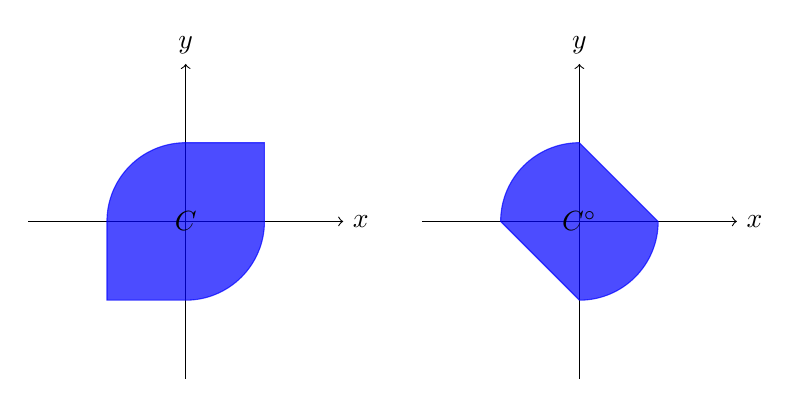
\begin{tikzpicture}
\draw[->, black] (-5,0) -- (-1,0) node[right]{$x$};
\draw[->, black] (-3,-2) -- (-3,2) node[above]{$y$};
\draw[fill, blue, opacity=0.7]
 (-3,1) arc (90 :180: 1) -- (-4,-1) -- (-3, -1) 
arc (270:360:1) -- (-2,1) -- cycle; 
\node[black] at (-3,0) {$C$};
\draw[->, black] (0,0) -- (4,0) node[right]{$x$};
\draw[->, black] (2,-2) -- (2,2) node[above]{$y$};
\draw[fill, blue, opacity=0.7]
 (2,1) arc (90 :180: 1) -- (2, -1) 
arc (270:360:1) -- cycle; 
\node[black] at (2,0) {$C^\circ$};
\end{tikzpicture}
}
\item $C=\left\{(x,y)\in\R^2\,\bigg|\,y\geq b+\frac{x^2}{2}\right\}
\; (b\in\R)$.\\
\bluea{
Notice that $C= \epi f$ where $f = b + \frac{x^2}{2}$. We have
$\bar x = \nabla f(\bar x)$. If $c < 0$, then 
$(d, c) = -c(-d/c, -1) = -c(\nabla f(-d/c), -1)\in N_{\epi f}(-d/c, 
f(-d/c))$ (see Section 3.2, Exercise 11). Thus, for all $(x,r)\in\epi f$, 
\begin{equation*}
d(x+\frac{d}{c}) + c(r - f\left(-\frac{d}{c}\right)) \leq 0.
\end{equation*}
In other words, 
\begin{equation*}
\max_{(x,r)\in\epi f} (d,c)^\top(x,r) = -\frac{d^2}{c} + cf\left(-
\frac{d}{c}\right) = c\left(b-\frac{d^2}{2c^2}\right).
\end{equation*}
Thus, when $c<0$, we have 
\begin{equation*}
(d,c)\in C^{\circ}\iff c\left(b-\frac{d^2}{2c^2}\right)\leq 1 
\iff d^2 \leq 2c(bc-1).
\end{equation*}
When $c>0$, then we can take $(x,r)$ with $r\to\infty$ to get that 
$(d,c)\notin C^{\circ}$, as $(d,c)^\top(x,r) > 1$. When $c=0$,
if $d\neq 0$, then we can take $x\to \infty$ with a suitable choice of 
$r$ or likewise with $x\to -\infty$ to make $(d,c)^\top (x,r) 
= dx \to +\infty$, so that $(d,0)\notin C^{\circ}$. On the other 
hand, if $(d,c) = 0$, then $(d,c)^\top (x,r) = 0 \leq 1$ for all 
$(x,r)$, so $0\in C^{\circ}$. Thus, 
\begin{equation*}
C^{\circ} = \{0\} \cup \{(d,c): c<0,\, d^2 \leq 2c(bc-1)\}
= \{(d,c) : c\leq 0,\, d^2 \leq 2c(bc-1)\}.
\end{equation*}
}
\end{enumerate}
\noindent
\textbf{4 (Polar sets and cones).} Suppose the set $C\subset\E$ is 
closed, convex, and contains 0. Prove the convex cones in $\E\times \R$
\begin{equation*}
\cl\R_+(C\times\{1\}) \text{ and } \cl\R_+(C^\circ\times\{-1\})
\end{equation*}
are mutually polar.
\bluea{
\begin{proof}
Notice the above two sets are cones, which means we are verifying they 
are each others' polar cones. As $S:=\cl\R_+(C\times\{1\})$ is a 
closed convex cone, by Theorem 3.1.8 (Bipolar cone), the bipolar equals 
itself, so we just need to verify that $T:=\cl\R_+(C^\circ\times\{-1\})$ 
equals $S^\circ=S^-$. \\
 For any set $A$, it 
turns out $A^\circ = (\cl A)^\circ$. Clearly $(\cl A)^\circ \subset 
A^\circ$. Now take $\phi\in A^\circ$. If $\tilde a \in \cl A$, then 
there is a sequence $a^i\to \tilde a$ in $A$, so 
$\ip{\phi, a^i} \leq 1$ for 
all $i\in\N$. Taking the limit, $\ip{\phi, \tilde a} \leq 1$, and since 
$\tilde a$ was arbitrary $\phi\in(\cl A)^\circ$. So $A^\circ \subset 
(\cl A)^\circ$, ergo $A^\circ = (\cl A)^\circ$. \\
\green{Actually, here is a proof that polar cones of $A,B$ with 
$\cl\conv\R_+A=\cl\conv\R_+B$ equal. $A^{--}=\cl\conv\R_+A$, and since 
$A^-$ is a closed convex cone, $A^- = A^{---}=(\cl\conv\R_+A)^-$.}
Thus,
denoting an element of $\R_+(C\times\{1\})$ as 
$c(x,1)$, where $c\geq 0$ and $x\in C$,
\begin{equation*}
(y,r)\in S^\circ \quad \iff \quad 
\forall c(x,1)\in \R_+(C\times\{1\}), \; c(\ip{x,y} + r) \leq 0
\; \iff \; \forall x\in C,\; \ip{x,y}+r\leq 0.`
\end{equation*}
If $r\neq 0$, we get for all $x\in C,\; 
-r(\ip{x,-y/r} -1) \leq 0$. If $r>0$, then we get $\forall x\in C,\; 
\ip{x, -y/r} \geq 1$. But this gives a contradiction, since we can 
take $x=0$ \green{(Kind of amazing that this is the only place where 
the assumption $0\in C$ is used)}.
 If $r<0$, then we have $\forall x\in C,\; \ip{x,-y/r} \leq 1$,
i.e. $-y/r\in C^\circ$. Moreover, if $-y/r\in C^\circ$, $\forall x\in C,
\; \ip{x,y}+r=-r(\ip{x,-y/r}-1)\leq 0$.
Thus, 
\begin{equation*}
r\neq 0:\; (y,r)\in X^\circ \iff r<0,\; -y/r\in C^\circ
\iff (y,r) \in \R_{++}(C^\circ\times\{-1\}).
\end{equation*}
On the other hand, if $r=0$, then we get $\forall x\in C,\; \ip{x,y} 
\leq 0$, i.e. $y\in C^-$. Thus, 
\begin{equation*}
S^\circ = \R_{++}(C^\circ \times \{-1\})\cup (C^-, 0).
\end{equation*}
Furthermore, by the inclusions 
\begin{equation*}
\cl\R_+(C^\circ\times\{-1\})\subset 
\R_{++}(C^\circ \times \{-1\})\cup (C^-, 0)\subset
\cl\R_+(C^\circ\times\{-1\}),
\end{equation*}
we have $S^\circ = T$ as desired. To verify the left inclusion, 
note that $\R_+(C^\circ \times \{-1\}) = \R_{++}(C^\circ\times\{-1\})
\cup \{0\}$, and $0\in (C^-, 0)$. Furthermore, $S^\circ$ is closed, which
gives the left inclusion. For the right inclusion, note that $\R_+C^- = C^-
\subset C^\circ$. Therefore, for $x^-\in C^-$, we can take 
$c^\circ(\frac{x^-}{c^\circ}, -1) = (x^-, c^\circ)
\in \R_+(C^\circ\times\{-1\})$ and take $c^\circ\to 0$ to obtain 
$(x^-, 0)\in (C^-, 0)$.\\
\green{Shorter proof, more opaque but maybe more elegant (wait actually
after writing it I think it's basically a more concise version of the 
above proof):
By the statement $\forall x\in C,\; \ip{x,x^\circ}-1\leq 0$ iff 
$x^\circ\in C^\circ$, we obtain 
\begin{equation*}
C^\circ\times\{-1\} = \{(y, -1): (y, -1)\in (C\times\{1\})^-\}.
\end{equation*}
Note that no element of the form
 $(y,1)$ exists in $(C\times\{1\})^-$,
since $(0, 1)\in C\times\{1\}$. Furthermore, for every element 
of the form $(y,0)\in (C\times\{1\})^-$, we can use convex conity 
of $(C\times\{1\})^-$ on $(y,0)$ and $(0, -1)$ and the fact that 
$\R_+y\subset C^-\subset C^\circ$ to obtain a 
sequence in $\R_+(C^\circ\times\{-1\})$ converging to $(y,0)$. Therefore, 
$(C\times\{1\})^- = \cl\R_+(C^\circ\times\{-1\})$. By an earlier 
comment, $(\cl\R_+(C\times\{1\}))^\circ = (C\times\{1\})^- = 
\cl\R_+(C^\circ\times\{-1\})$, and $\cl\R_+(C\times\{1\})$ is self-bipolar,
which finishes the proof.
}
\end{proof}}
\noindent
\textbf{5 * (Polar sets).} Suppose $C$ is a nonempty subset of $\E$. 
\begin{enumerate}[(a)]
\item Prove $\gamma_C^* = \delta_{C^\circ}$. \\
\bluea{
Let $y\notin C^\circ$. Thus, there exists $x\in C$ such that 
$\ip{y,x} > 1$. Now, for all $\lambda\in\R_+$,
\begin{equation*}
(\gamma_C)^*(y) = \sup_{x'\in \E}\ip{y,x'}-\gamma_C(x') 
\geq \ip{y, \lambda x} - \gamma_C(\lambda x)  = \lambda(\ip{y,x}
- \gamma_C(x)).
\end{equation*}
By taking $\lambda\to+\infty$, we see $(\gamma_C)^*(y) = +\infty$.
Now suppose $y\in C^\circ$ and take $x\in \E$. If $\not\exists 
\lambda\in\R_+$ such that $x\in \lambda C$, then $\ip{y,x} - 
\gamma_C(x) = -\infty$. Otherwise, let $\bar\lambda = \gamma_C(x)$. 
If $x = \bar\lambda x_C$ for some $x_C\in C$,
\begin{equation*}
\ip{y, \bar\lambda x_C} - \gamma_C(\bar\lambda x_C) = \bar\lambda(\ip{y,x_C}
- \gamma_C(x_C)) \leq 0,
\end{equation*}
because $\ip{y, x_C}\leq 1$, and if $\gamma_C(x_C) < 1$, then for some 
$\lambda < 1$, $x_C\in\lambda C \implies x\in\bar\lambda\lambda C$, 
contradicting minimality of $\bar\lambda$. Now if $x\neq \bar\lambda x_C$
for any $x_C\in C$, there is still a sequence $\lambda^i, x_C^i$ 
where $\lambda^i > \bar\lambda, \, \lambda^i \to \bar\lambda$, and 
$x=\lambda^i x_C^i$. Now $\gamma_C(x^i_C) \geq
 \frac{\bar\lambda}{\lambda^i}$,
because if $\gamma_C(x^i_C) < \frac{\bar\lambda}{\lambda^i}$, then 
$x = \lambda^i x^i_C = \lambda x_C'$ for some $\lambda < \bar\lambda$ 
and $x_C'\in C$, contradicting minimality of $\bar\lambda$. Thus, 
\begin{equation*}
\ip{y,x} - \gamma_C(x) = \lambda_i(\ip{y, x^i} - \gamma_C(x^i))
\leq \lambda_i(1-\frac{\bar\lambda}{\lambda^i}).
\end{equation*}
If $\bar\lambda > 0$, then since $\lambda^i\to\bar\lambda$, the RHS 
goes to 0. If $\bar\lambda = 0$, then the RHS still goes to 0 because 
of the factor $\lambda_i \to 0$. Thus, $\ip{y,x} - \gamma_C(x) \leq 0$.
Since $x$ was arbitrary, we have shown 
\begin{equation*}
y\in C^\circ \implies (\gamma_C)^*(y) = 0.
\end{equation*}
This completes the proof that $(\gamma_C)^*=\delta_{C^\circ}$.
\green{God this question was annoying.}
}
\item Prove $C^\circ$ is a closed convex set containing $0$.  \\
\bluea{
$C^\circ$ is closed because it is an intersection of closed sets
(specifically, halfspaces):
\begin{equation*}
C^\circ = \bigcap_{x\in\E} \{\phi\in \E: \ip{\phi, x}\leq 1\}.
\end{equation*}
Finally, by the above, it is also an intersection of convex sets
containing 0.
}
\item Prove $C\subset C^{\circ\circ}$.  \\
\bluea{
Take $\phi\in C^\circ$ and $x\in C$. By definition, $\ip{\phi, x}\leq 1$.
But, $\phi$ was arbitrary, so in fact $x\in C^{\circ\circ}$.
}
\item If $C$ is a cone, prove $C^\circ = C^-$. \\
\bluea{
If $\ip{\phi, x} > 0$ for some $x\in C$, by scaling we have 
$\ip{\phi, cx}>1$ for some $cx\in C$. Thus, if $\phi\in C^\circ$, 
$\phi\in C^-$, so $C^\circ\subset C^-$. The reverse inclusion is clear.
}
\item For a subset $D$ of $\E$, prove $C\subset D$ implies 
$D^\circ \subset C^\circ$. \\
\bluea{
Suppose $\phi\in D^\circ$. Then, if $x\in C$, since $x\in D$, we have 
$\ip{\phi, x}\leq 1$. Since $x\in C$ was arbitrary, $\phi\in C^{\circ}$.
}
\item Prove $C$ is bounded if and only if $0\in\inter C^\circ$.  \\
\bluea{
If $C$ is bounded, then there exists $M>0$ such that $\|x\|\leq M$ 
for all $x\in C$. Then, if $\|\phi\|\leq M^{-1}$, we have 
$\ip{\phi, x}\leq \|\phi\|\|x\|\leq 1$ for all $x\in C$, i.e. 
$\phi\in C^{\circ}$. Thus, $M^{-1}B\in C^\circ$, i.e. $0\in\inter
 C^\circ$.\\
Now if $C$ is unbounded, there exists a sequence $x^i$ with unbounded 
norm. For any $\epsilon > 0$, $\sup_{\phi\in\epsilon B} \ip{\phi, x^i} 
= \epsilon \|x^i\|\to +\infty$. Therefore, $0\notin \inter C^\circ$.
}
\item For any closed halfspace $H\subset\E$ containing 0, prove 
$H^{\circ\circ} = H$.  \\
\bluea{
$H$ takes the form $\{x: \ip{a, x} \leq b\}$ for some $b\geq 0$.
If $\phi\neq 0$ is not a multiple of $a$, then it has a component 
perpendicular to $a$, $v$. The point $cv\in H$ for $c>0$ large enough 
gives $\ip{\phi, cv} > 1$, meaning $\phi\notin H^\circ$. Now if 
$\phi = ca$ for some $c\geq 0$, for any $x\in H$ we have 
$\ip{ca, x} \leq cb$, with equality when $x=\frac{b a}{\|a\|^2}$.
 If $c<0$ then we can 
take $x=-la\in H$, $l\to+\infty$ to get $\ip{ca, -la} > 1$. 
Thus, $C^\circ = \{ca: 0\leq c \leq b^{-1}\}$ If $b=0$, then replace 
$b^{-1}$ with $+\infty$.\\
Now take $x\in \E$.
\begin{equation*}
\ip{x, ca} = c\ip{x,a} \leq 1 \; \forall 0\leq c\leq b^{-1}
\; \iff \; \ip{x,a}\leq b.
\end{equation*}
Thus, $H^{\circ\circ}=H$.
}
\item Prove Theorem 4.1.5 (Bipolar set). \\
\bluea{
By parts (b) and (c), $C^{\circ\circ}$ is closed, convex, and contains 
0, and $C\subset C^{\circ\circ}$. Therefore, $\cl(\conv(C\cup\{0\}))
\subset C^{\circ\circ}$. \\
Now take $y\notin \cl(\conv(C\cup\{0\}))$. By Theorem 2.1.6 (Basic 
separation), there exist $a\in \E$ and $b\in\R$ such that 
\begin{equation*}
\forall x\in \cl(\conv(C\cup\{0\})),\;\ip{a,x}\leq b < \ip{a,y}.
\end{equation*}
Now if $b<0$, then we get a contradiction since we can take $x=0$.
Thus, $b\geq 0$. If $b=0$, then we can replace $b$ with $2^{-1}(b+ 
\ip{a,y})$, allowing us to assume $b>0$. Then, 
\begin{equation*}
\forall x\in\cl(\conv(C\cup\{0\})),\; \ip{\frac{a}{b}, x}\leq 1
< \ip{\frac{a}{b},y}.
\end{equation*}
Since $C\subset \cl(\conv(C\cup\{0\}))$, we have $\frac{a}{b}\in C^\circ$.
Yet, $\ip{\frac{a}{b},y} > 1$. Thus, $y\notin C^{\circ\circ}$. This 
completes the proof that $C^{\circ\circ}=\cl(\conv(C\cup\{0\}))$.
}
\end{enumerate}
\noindent
\textbf{6 * (Polar sets and strict separation).} Fix a nonempty 
set $C\in\E$. 
\begin{enumerate}[(a)]
\item For points $x\in\inter C$ and $\phi\in C^\circ$, prove 
$\ip{\phi, x}\leq 1$.\\
\bluea{
Since $x\in\inter C$, for some $\epsilon > 0,\; x+\epsilon B\subset C$. 
Thus, if $\phi=0$, the inequality is obviously true, and otherwise,
\begin{equation*}
\ip{x+\epsilon\frac{\phi}{\|\phi\|}, \phi} \leq 1 
\implies \ip{x,\phi} \leq 1 - \epsilon\|\phi\| < 1.
\end{equation*}
}
\item Assume further that $C$ is a convex set. Prove $\gamma_C$ is 
sublinear. \\
\bluea{
First we prove that $\gamma(\mu x)=\mu\gamma(x)$ for $\mu 
\in\R_+$. If $\mu>0$, then for any $\lambda\in\R_+$,
\begin{equation*}
x\in\lambda C \iff \mu x \in \lambda\mu C 
\implies \gamma_C(\mu x) = \mu\gamma_C(x).
\end{equation*}
If $\mu=0$, then $\gamma(\mu x) = \gamma(0) = 0$, since $0\in 0C$.
Note that as we just showed, positive homogeneity does not require 
convexity of $C$. \\
Now we show subadditivity, which goes on to imply sublinearity. For 
$x_1$ and $x_2$ in $\E$, suppose $x_1\in\lambda_1 C$ and $x_2 \in 
\lambda_2 C$ for $\lambda_1,\lambda_2\geq 0$. If $\lambda_1=\lambda_2=0$, 
then $x_1= x_2 = 0$ (since $0C=\{0\}$), so $x_1+x_2 = 0 \in (\lambda_1+\lambda_2)
C = 0C$. Otherwise, 
\begin{equation*}
x_1 + x_2 \in \lambda_1 C+\lambda_2 C = 
(\lambda_1+\lambda_2)\left(\frac{\lambda_1}{
\lambda_1+\lambda_2}C + \frac{\lambda_2}{\lambda_1+\lambda_2}C\right)
\subset (\lambda_1+\lambda_2)C,
\end{equation*}
by convexity of $C$. Therefore, if $\gamma_C(x_1) < r_1$ and 
$\gamma_C(x_2)<r_2$, then for some $0\leq \lambda_1<r_1,\,
 0\leq \lambda_2<r_2,\; x_1\in\lambda_1 C$ and $x_2\in\lambda_2 C$, 
so $x_1 + x_2 \in (\lambda_1+\lambda_2)C$. Thus, $\gamma_C(x_1+x_2)
< r_1+r_2$. So, taking an infimum over $r_1$ and then $r_2$, 
\begin{gather*}
\forall r_2 > \gamma_C(x_2), \;
\gamma_C(x_1+x_2) \leq \inf\{r_1>\gamma_C(x_1)\} + r_2 \\
\implies \gamma_C(x_1+x_2)\leq \inf\{r_1>\gamma_C(x_1)\} + \inf\{r_2
> \gamma_C(x_2)\} = \gamma_C(x_1)+\gamma_C(x_2).
\end{gather*}
\green{Surprisingly hard to justify that if $x \leq r_1+r_2$ for 
all $r_1\in R_1$ and $r_2\in R_2$, then $x\leq \inf R_1 + \inf R_2$
XD}
}
\item Assume in addition $0\in\core C$. Deduce 
\begin{equation*}
\cl C = \{x \mid \gamma_C(x)\leq 1\}.
\end{equation*} 
\bluea{
Since $0\in\core C$, $\gamma_C$ is everywhere finite and therefore 
continuous, by Theorem 4.1.3 (Convexity and continuity). Suppose 
$x\in \cl C$. Then, there exists a sequence $x^i \to x$ in $C$. 
By continuity, $\gamma_C(x^i)\to \gamma_C(x)$. Since $\gamma_C(x^i)
\leq 1$ for all $i\in\N$, $\,\gamma_C(x)\leq 1$. \\
Now suppose $\gamma_C(x)\leq 1$. Then, there is a 
decreasing sequence $\mu^i\to 1$ such that $x\in \mu^i C$ for every 
$i\in\N$, i.e. $\frac{x}{\mu^i} \in C$. Since $\mu^i\to 1$, we have 
$\frac{x}{\mu^i} \to x$, which proves $x\in \cl C$.
}
\item Finally, suppose in addition that $D\subset\E$ is a convex set 
disjoint from the interior of $C$. By considering the Fenchel program 
$\inf\{\delta_D+\gamma_C\}$, prove there is a closed halfspace containing
$D$ but disjoint from the interior of $C$. \\
\bluea{
Note that $\inf\{\delta_D + \gamma_C\} \geq 1$, since if $x\in D$, 
$\gamma_C(x)\geq 1$ (the proof of Theorem 4.1.4 (Core and interior) 
shows that $\inter C = \{x\mid \gamma_C(x) < 1\}$, which is disjoint 
from $D$ by assumption). \\
Since $\dom\gamma_C = \E$, the primal and dual Fenchel problems have 
equal value, with achievement for the dual (see Theorem 3.3.5, 
Fenchel duality): 
\begin{align*}
1\leq \inf_{x\in\E}\{\gamma_C(x)+\delta_D(x)\} &= \sup_{\phi\in\E}\{
-\gamma_C^*(\phi) - \delta_D^*(-\phi)\} \\
&= \sup_{\phi\in\E}\{-\delta_{C^\circ}(\phi) - \sup_{x\in D}\ip{-\phi, x}
\} \\
&= \sup_{\phi\in C^\circ}\inf_{x\in D}\ip{\phi, x}.
\end{align*}
In the second line we used $\gamma_C^*=\delta_{C^\circ}$, from part 
(a) of Exercise 5. The sup is achieved, so there exists $\phi\in C^\circ$
such that $\forall x\in D,\, \ip{\phi, x} \geq 1$. But since 
$\phi\in C^\circ$, for any $x\in \inter C$, we have $\ip{\phi, x} < 1$.
We have found our closed halfspace:
\begin{equation*}
H= \{x\in \E: \ip{\phi, x}\geq 1\}\text{ satisfies }
D\subset H \text{ and } D\cap \inter C = \emptyset.
\end{equation*}
\green{Wow Fenchel duality is op.}
}
\end{enumerate}
\noindent
\textbf{7 * (Polar calculus [23]).} Suppose $C$ and $D$ are subsets of 
$\E$.
\begin{enumerate}[(a)]
\item Prove $(C\cup D)^\circ = C^\circ\cap D^\circ$. 
\bluea{
\begin{align*}
\phi\in(C\cup D)^\circ & \iff \forall x \in C,\; \ip{\phi, x}\leq 1 
\text{ and }\forall x\in D,\;\ip{\phi, x} \leq 1 \\
&\iff \phi \in C^\circ\cap D^\circ.
\end{align*}
}
\item If $C$ and $D$ are convex, prove 
\begin{equation*}
\conv(C\cup D) = \bigcup_{\lambda\in[0,1]} (\lambda C + (1-\lambda)D).
\end{equation*} 
\bluea{
The $\supset$ inclusion holds almost by definition: for any 
$\lambda\in[0,1]$ and $c\in C,\, d\in D,\, \lambda c + (1-\lambda) d
\in \conv(C\cup D)$ because $c\in \conv(C\cup D)$ and $d\in\conv(C
\cup D)$ and $\conv(C\cup D)$ is convex. \\
For $\subset$, we show that $\bigcup_{\lambda\in[0,1]}(\lambda C + 
(1-\lambda)D)$ is convex. Clearly, it contains $C\cup D$. Since 
$\conv(C\cup D)$ is the smallest convex set containing $C\cup D$, 
the inclusion follows. To see convexity, first note the sets 
$[0,1](C\times\{1\})$ and $[0,1](D\times\{1\})$ are convex: for any 
nonnegative interval $[a,b]$ and convex set $\bar C$, the set 
$[a,b]\bar C$ is convex, since $a\leq\alpha,\beta\leq b$ and 
$x_1,x_2\in \bar C$, $\lambda\in[0,1]$ implies 
\begin{equation*}
\lambda\alpha x_1 + (1-\lambda)\beta x_2 
= (\lambda\alpha+(1-\lambda)\beta)\left(\frac{\lambda\alpha}{
\lambda\alpha+(1-\lambda)\beta} x_1 + \frac{(1-\lambda)\beta}{
\lambda\alpha+(1-\lambda)\beta}x_2\right) \in [a,b]\bar C.
\end{equation*}
If $\lambda\alpha+(1-\lambda)\beta = 0$, then $\lambda\alpha = 
(1-\lambda)\beta = 0$ and either $\alpha$ or 
$\beta=0$, so $\lambda\alpha x_1 + (1-\lambda)\beta x_2 = 0 \in 
[a,b]\bar C = [0,b]\bar C$. \\
Now, notice that $g:= \delta_{[0,1](C\times\{1\})}\odot\delta_{[0,1]
(D\times\{1\})}$ is convex (3.3 Exercise 12(a)) and
\begin{align*}
g(y,1)&=\inf_{(x,\lambda) \in\E\times\R} \delta_{[0,1](C\times\{1\})}(x,
\lambda)
+ \delta_{[0,1](D\times\{1\})}(y-x, 1-\lambda) \\
&= \delta_{\bigcup_{\lambda\in[0,1]}(\lambda C + (1-\lambda)D)}(y).
\end{align*}
In other words, $\bigcup_{\lambda\in[0,1]}\lambda C + (1-\lambda)D$
is the $\E$ part of
$\dom g$, which is convex.
Thus, $\bigcup_{\lambda\in[0,1]}
\lambda C + (1-\lambda)D$ is convex.
}
\item If $C$ is a convex cone and the convex set $D$ contains 0, prove 
\begin{equation*}
C+D \subset \cl\conv(C\cup D).
\end{equation*} 
\bluea{
Consider $c+d\in C+D$. Take a sequence $\lambda^i \to 0$. We have 
$\lambda^i\frac{c}{\lambda^i} + (1-\lambda^i) d \to c + d$.
Notice the LHS is in $\bigcup_{\lambda\in[0,1]}(\lambda C + (1-\lambda)D)
= \conv(C\cup D)$. Therefore, $c+d\in \cl(\conv(C\cup D))$.
}
\end{enumerate}
Now suppose the closed convex sets $K$ and $H$ of $\E$ both contain 0. 
\begin{enumerate}[(a),resume]
\item Prove $(K\cap H)^\circ = \cl\conv(K^\circ\cup H^\circ)$. \\
\bluea{
By part (a), $(K^\circ \cup H^\circ)^\circ = K^{\circ\circ}\cap 
D^{\circ\circ}=K\cap H$. The second equality is by Theorem 4.1.5
 (Bipolar set) \eqref{4.1.5} Since $K$ and $H$ 
already are closed, convex, and contain 0, they are self bipolar. 
Now we take another polar and apply Theorem 4.1.5 again: 
\begin{equation*}
(K^\circ\cup H^\circ)^{\circ\circ} = \cl\conv(K^\circ \cup H^\circ)
= (K\cap H)^\circ.
\end{equation*}\vspace{-0.3in}
}
\item If furthermore $K$ is a cone, prove $(K\cap H)^\circ = 
\cl(K^\circ + H^\circ)$.\\
\bluea{
Note 
$\conv(K^\circ\cup H^\circ) \subset K^\circ + H^\circ$. This is because 
by part (b), an element of $\conv(K^\circ\cup H^\circ)$ is 
$\lambda k + (1-\lambda)h$ for some $\lambda\in[0,1],\,k\in K^\circ,\,
h\in H^\circ$, which is in $K^\circ + H^\circ$ because both sets 
contain 0. 
Thus, $\cl\conv(K^\circ\cup H^\circ)\subset \cl(K^\circ + H^\circ)$.
Part (c) shows the reverse inclusion. Thus, by the previous part,
\begin{equation*}
(K\cap H)^\circ = \cl(\conv(K^\circ\cup H^\circ))
= \cl(K^\circ + H^\circ).
\end{equation*}
}
\end{enumerate}
\noindent
\textbf{8 ** (Polar calculus [23]).} Suppose $P$ is a cone in $\E$ and 
$C$ is a nonempty subset of a Euclidean space $\Y$. 
\begin{enumerate}[(a)]
\item Prove $(P\times C)^\circ = P^\circ\times C^\circ$.\\
\bluea{
$P^\circ\times C^\circ\subset (P\times C)^\circ$, since if 
$\ip{p^\circ, p}\leq 1$ for all $p\in P$ and $\ip{c^\circ, c}\leq 1$ 
for all $c\in C$, then since $P$ is a cone (cones are nonempty, 
see page 1 of the textbook), $\ip{p^\circ, p}\leq 0$ 
for all $p\in P$, and 
\begin{equation*}
\forall p, c \in P\times C,\;
\ip{(p^\circ, c^\circ), (p, c)} = \ip{p^\circ, p} + \ip{c^\circ, c}
\leq 1.
\end{equation*}
$(P\times C)^\circ\subset P^\circ\times C^\circ$ because if $(a,b)
\in (P\times C)^\circ$, then since $0\in P$,
\begin{equation*}
\forall c\in C,\, \ip{(a,b), (0,c)} = \ip{b,c} \leq 1,
\end{equation*}
so $b\in C^\circ$. Furthermore,
\begin{equation*}
\forall p\in P,\, \ip{(a,b), (p,c)} = \ip{a,p} + \ip{b,c} \leq 1.
\end{equation*}
If $P$ contains a nonzero element $p$, then, we must have 
$\ip{a,p} \leq 0$. Thus, $(a,b)\in P^\circ\times C^\circ$.
}\vspace{-0.1in}
\item If furthermore $C$ is compact and convex (possibly not containing 
$0$), and $K$ is a cone in $\E\times\Y$, prove 
\begin{equation*}
(K\cap (P\times C))^\circ = (K\cap (P\times C^{\circ\circ}))^\circ.
\end{equation*}
\bluea{
$K\cap (P\times C) \subset K\cap (P\times C^{\circ\circ})$,
so $(K\cap (P\times C^{\circ\circ}))^\circ\subset 
(K\cap (P\times C))^\circ $ (See Exercise 5 (e)). \\
Now take $(\phi,\psi)\in (K\cap (P\times C))^\circ$. Consider 
an element $(a,b)\in K\cap (P\times C^{\circ\circ})$. By compactness 
of $C$ and Section 2.2 Exercise 5 (d) which says that the convex 
hull of a compact set is compact,
\begin{equation*}
C^{\circ\circ} = \cl(\conv(C\cup\{0\})) = \conv(C\cup\{0\})
= \bigcup_{\lambda\in[0,1]} \lambda C.
\end{equation*}
The last equality follows from Exercise 7, part (b). Therefore, 
$(a,b) = (p, \lambda c)$ for some $\lambda\in[0,1]$ and $c\in C$. 
If $\lambda > 0$, then $(\frac{p}{\lambda}, c)\in K\cap (P\times C)$.
 Thus, 
\begin{equation*}
\ip{(\phi,\psi),(p, \lambda c)} = 
\lambda\ip{(\phi, \psi), (\frac{p}{\lambda}, c)} \leq \lambda\leq 1.
\end{equation*}
If $\lambda =0$, we can take a sequence $\lambda^i\to \lambda$ 
such that $\ip{(\phi,\psi), (p,\lambda^i c)}\leq 1$, which proves 
that $\ip{(\phi, \psi), (p, 0)} \leq 1$. Therefore, $(\phi, \psi)
\in (K\cap (P\times C^{\circ\circ}))^{\circ}$.
}
\item If furthermore $K$ and $P$ are closed and convex, use Exercise 7 to 
prove 
\begin{equation*}
(K\cap (P\times C))^\circ = \cl(K^\circ + (P^\circ\times C^\circ)).
\end{equation*}
\bluea{
By Exercise 7(e), since $(P\times C^{\circ\circ})$
 is now closed and convex and contains 0, and $K$ is a closed convex 
cone, 
\begin{equation*}
(K\cap (P\times C))^\circ = 
(K\cap (P\times C^{\circ\circ})) = 
\cl(K^\circ + (P\times C^{\circ\circ})^\circ)
= \cl (K^\circ + (P^\circ\times C^{\circ})),
\end{equation*}
using parts (a) and (b).
}
\item Find a counterexample to part (c) when $C$ is unbounded. \\
\bluea{
Let $P=\{0\}, C = \{(1, r): r\geq 0\}$, and $K=\{0\}\times\{(0, r):
r\geq 0\}$. $P$ and $K$ are closed, convex cones, and $C$ is a closed,
convex set. Since basically only the $\Y$ space is relevant here, 
let's plot $C$ and $K_\Y$, the projection of $K$ onto its $\Y$ 
component, as well as their polars.\\
\begin{tikzpicture}
\draw[->, black] (-5,0) -- (-1,0) node[right] {$x$};
\draw[->, black] (-3,-2) -- (-3, 2) node[above] {$y$};
\draw[thick] (-3,0) -- (-3, 1.98) node[below left] {$K_\Y$};
\draw[thick, orange] (-2,0) -- (-2, 1.98) node[below right] {$C$};
\draw[->, black] (0,0) -- (4,0) node[right] {$x$};
\draw[->, black] (2,-2) -- (2, 2) node[above] {$y$};
\draw[ultra thick, fill, opacity=0.7] (0.1,0)--(3.9,0)
node[above left] {$K_\Y^\circ$}
--(3.9,-2)--(0.1,-2)--cycle;
\draw[fill,orange, opacity=0.6] 
(0.1,0)--node[above, pos=0.5] {$C^\circ$} (2.9,0)--(2.9,-2)--(0.1,-2)--cycle;
\end{tikzpicture}\\
As shown, $C^\circ = \{(1,y): y\geq 0\}^\circ = \{(x,y): x\leq 1,\; 
y \leq 0\}$. If $y\geq 0$ and $x\leq 1,\, y'\leq 0$, then 
$\ip{(1,y), (x,y')} = x + yy' \leq x \leq 1$. Conversely, if 
$x>1$, then $\ip{(1,0),(x,y)} = x > 1$ and if $y'>0$, then by 
choosing $y$ large enough, $\ip{(1,y),(x,y')} = x+yy' > 1$. \\
Now notice $(K\cap (P\times C))^\circ = (\emptyset)^\circ = \E\times\Y$.
On the other hand, 
\begin{align*}
\cl(K^\circ + (P^\circ\times C^\circ))
&= \cl((\E\times\{(x,y):y\leq 0\})
 + (\E\times\{(x,y):x\leq 1,\, y\leq 0\}))\\
&\subset \E\times\{(x,y): y\leq 0\}\neq \E\times \Y = (K\cap (P\times C))^{
\circ}.
\end{align*}
\vspace{-0.2in}
}
\end{enumerate}
\noindent
\textbf{9 * (Open mapping theorem).} Suppose the linear map $A:\E\to\Y$ 
is surjective. 
\begin{enumerate}[(a)]
\item Prove any set $C\in\E$ satisfies $A\core C\subset \core AC$. \\
\bluea{
Take $x\in \core C$. Since $A$ is surjective, for any $d\in \Y$,
there exists $y\in \E$ such that $Ay=d$. For some $\epsilon > 0$, 
$x+\epsilon y\in C$. Thus, $A(x+\epsilon y) = Ax +\epsilon d\in AC$. 
Since $d$ was arbitrary, $Ax\in\core AC$. Thus, $A\core C\subset 
\core AC$.
}
\item Deduce $A$ is an \text{open map}: that is, the image of any open 
set is open. \\
\bluea{
Linear maps map convex sets to convex sets: if
$z_1=Ax_1$ and $z_2=Ax_2$, then $\lambda z_1 + (1-\lambda)z_2 
= A(\lambda x_1 + (1-\lambda)x_2)$.\\
Now if $C$ is an arbitrary open set, take a point 
$x\in\inter C$. For some $\epsilon > 0,\, \tilde B:= 
x+\epsilon B\subset C$. $\tilde B$ is convex, and so $A\tilde B
\subset AC$ is convex. Since $x\in\core\tilde B,\, Ax\in\core 
A\tilde B = \inter A\tilde B$ by Theorem 4.4 (Core and interior).
There is a ball around $Ax$ in $A\tilde B$, and thus $AC$. Thus, 
$AC$ is open.
}
\item Prove another condition ensuring condition (3.3.8) in the Fenchel
theorem is that there is a point $\hat x$ in $\inter(\dom f)$ with 
$A\hat x$ in $\dom g$ and $A$ is surjective. Prove similarly that a 
sufficient condition for Fenchel duality with linear constraints 
(Corollary 3.3.11) to hold is $A$ surjective and $b\in A(\inter(\dom f))$.\\
\bluea{
The condition (3.3.8) is $0\in\core(\dom g - A\dom f)$. Since by 
part (a), $A\core(\dom f) = \core(A\dom f)$, $A\hat x\in\core(A
\dom f)\cap \dom g$. Thus, we can take this to be our point in 
$\dom g$, and for any direction find a point in $A\dom f$ which is 
strictly in that direction relative to $A\hat x$, proving 
$0\in \core(\dom g - A\dom f)$. \\
Now the sufficient condition of Corollary 3.3.11 is $b\in\core(A
\dom f)$. But by part (a), this is the same as $b\in A\core(\dom f)$.
By Theorem 4.4 (Core and interior) and convexity of $\dom f$,
 this is the same as $b\in A\inter(\dom f)$.
}
\item Deduce that any cones $H\subset\Y$ and $K\subset\E$, and any 
surjective linear map $A:\E\to\Y$ satisfy $(K\cap A^{-1}H)^- = A^*H^-
+ K^-$, providing $H\cap A(\inter K)\neq \emptyset$. \\
\bluea{
I think this should really have the hypothesis that $H$ and $K$ are 
convex, or else you can make $(K\cap H)^- = \{(x,y):y\leq 0\}$ 
and $H^- + K^- = \{(x,y): |x|\leq -y\}$, by making $K$ a convex 
cone centered on the positive $y$ axis of angle less than 90, 
and $H$ a cone which has a ray along the positive $y$ axis and 
the two rays whose union is $\{(x,y): |x|=y\}$. $H\cap K$ here 
would just be the positive $y$ axis. \\
Anyways, a sufficient condition for Theorem 3.3.13 (Krein-Rutman
polar cone calculus) is $H-AK=\Y$. If $H\cap A(\inter K)\neq \emptyset$,
then $H\cap \inter(AK)\neq \emptyset$. By choosing an element of 
$AK$ which differs from the interior element in an arbitrary 
direction and scaling, we get $H-AK=\Y$.
}
\end{enumerate}
\noindent
\textbf{10 * (Conical absorption)}
\begin{enumerate}[(a)]
\item If the set $A\subset\E$ is convex, the set $C\subset\E$ is bounded,
and $\R_+A=\E$, prove there exists a real $\delta > 0$ such that 
$\delta C\subset A$.\\
\bluea{
If $\R_+A=\E$, then the gauge function $\gamma_A$ is finite everywhere
and continuous. Because $C$ is bounded, it is contained in some closed
ball $MB$, on which $\gamma_A$ obtains a maximum. Note that if 
$\gamma_A(x)\leq \mu$, then $x\in \mu A$, since there exists 
$\lambda < \mu$ where $x\in \lambda A$, and by $\R_+A=\E$ and 
$A$ convex, $A$ must contain 0, so $\lambda A \subset \mu A$. 
Thus, $C\subset MB \subset (\max_{x\in MB}\gamma_A(x))A$.  
If $(\max_{x\in MB}\gamma_A(x))=0$ we can set $\delta$ to anything,
otherwise take $\delta = (\max_{x\in MB}\gamma_A(x))^{-1}$.
}
\end{enumerate}
Now define two sets in $\S_+^2$ by 
\begin{align*}
&A = \left\{\begin{bmatrix} y & x \\ x & z \end{bmatrix}\in \S_+^2\,\bigg|
\, |x|\leq y^{2/3}\right\}, \text{ and }\\
&C = \{X\in\S_+^2 \mid \tr X\leq 1\}.
\end{align*}
\begin{enumerate}[(a),resume]
\item Prove that both $A$ and $C$ are closed, convex, and contain $0$, 
and that $C$ is bounded. \\
\bluea{
$A$ is convex: note $y\geq 0$, because the corresponding matrix is 
PSD. Take two matrices in $A$, differentiating their entries by 
indexing those of one by 1 and those of the other by 2. $\S_+^2$ 
is convex, so any convex combination of them is still PSD. 
Also, for $\lambda\in[0,1]$, by convexity of $x\mapsto |x|^{3/2}$,
\begin{equation*}
|\lambda x_1 + (1-\lambda)x_2|^{3/2} \leq \lambda|x_1|^{3/2}+(1-\lambda)
|x_2|^{3/2} = \lambda y_1 + (1-\lambda)y_2.
\end{equation*}
Thus, raising both sides to the power $2/3$, we get that the convex 
combination is in $A$. Thus, $A$ is convex. It contains 0 as 
$|0|\leq 0^{2/3}$ and $0\in \S_+^2$. It is closed because 
$f\left(\begin{bmatrix} y & x \\ x & z \end{bmatrix}\right) = 
|x|-y^{2/3}$ is continuous, and so $\{X: f(X) \leq 0\}$ is closed. \\
$\tr$ is a linear functional, so $C$ is the intersection of 
$\S_+^2$ with the closed halfspace $\{X\in \S^2|\tr X\leq 1\}$, 
which makes it closed and convex. It contains 0 because 
$0\in\S_+^2$ and $\tr 0 = 0 \leq 1$. $C$ is bounded because 
\begin{equation*}
X\in C\implies \|X\| = \|\lambda(X)\| \leq \sum_{i=1}^n |\lambda_i(X)|
= \tr X \leq 1.
\end{equation*}
}\vspace{-0.2in}
\item Prove $\R_+A = \S_+^2 = \R_+C$. \\
\bluea{
For any nonzero $X\in \S_+^2$, $X/\tr X \in C$. Further, 
any positive scaling of $C$ is in $\S_+^2$. Thus, $\S_+^2 
= \R_+C$. Likewise, any positive scaling of $A$ is in $\S_+^2$ 
(this follows from the fact that $\S_+^2$ is a cone). \\
Now given $X=\begin{bmatrix} y & x \\ x & z \end{bmatrix}\in\S_+^2$, 
for any $c>0$, 
\begin{equation*}
|cx| \leq (cy)^{2/3} \iff c^{1/3}x\leq y^{2/3}.
\end{equation*}
We can clearly take a $c$ small enough so that $c^{1/3}x\leq y^{2/3}$. 
Thus, $c X \in A$. Thus, $X\in c^{-1} A$. This proves that 
$\S_+^2 = \R_+ A$.
}
\item Prove there is no real $\delta > 0$ such that $\delta C\subset A$.
\\
\bluea{Let $\delta >0$ be arbitrary and 
consider the following matrix in $\delta C$ for some $\lambda\in(0,1)$:
\begin{equation*}
X = \begin{bmatrix}
\delta \lambda & \delta\sqrt{\lambda(1-\lambda)} \\
\delta\sqrt{\lambda(1-\lambda)} & \delta(1-\lambda).
\end{bmatrix}
\end{equation*}
Its determinant is 0 and has trace $\delta$, so it belongs to 
$\delta C$. Let us compute when $X$ is not in $A$:
\begin{gather*}
\delta\sqrt{\lambda(1-\lambda)} > (\delta \lambda)^{2/3} 
\iff \delta^6 (\lambda(1-\lambda))^3 > \delta^4 \lambda^4 
\iff \delta^2 > \frac{\lambda}{(1-\lambda)^3}.
\end{gather*}
If we take $\lambda\to 0$, then $\frac{\lambda}{(1-\lambda)^3} 
\to 0 < \delta$. Therefore, there exists a setting of $\lambda$ 
for which $X\in \delta C$ yet $X\notin A$, proving 
$\delta C\not\subset A$.}
\end{enumerate}
\noindent 
\textbf{11 * (H\"{o}lder's inequality).} This question develops an 
alternative approach to the theory of the $p$-norm $\|\cdot\|_p$ defined 
in Section 2.3, Exercise 6. 
\begin{enumerate}[(a)]
\item Prove $p^{-1}\|x\|_p^p$ is a convex function, and deduce the 
set 
\begin{equation*}
B_p = \{x\mid \|x\|_p \leq 1\}
\end{equation*}
is convex. \\
\bluea{
Since the function $x\mapsto |x|^p$ is convex with derivative 
$x|x|^{p-2}$ (see Section 3.1 Exercise 14), the function 
\begin{equation*}
\frac{\|x\|_p^p}{p} = \frac{1}{p} \sum_{i=1}^n |x_i|^p 
\end{equation*}
is a sum of convex function and is thus convex, and has gradient 
$x|x|^{p-2}$ (where the multiplication and absolute value are 
element-wise). Then, $B_p$ is a level set of a convex function, 
which makes it convex.
}
\item Prove the gauge function $\gamma_{B_p}(\cdot)$ is exactly 
$\|\cdot\|_p$, and deduce $\|\cdot\|_p$ is convex.  
\bluea{
\begin{equation*}
\|\lambda x\|_p = \left(\sum_{i=1}^n |\lambda x_i|^p\right)^{1/p}
= \left(|\lambda|^p\sum_{i=1}^n |x_i|^p\right)^{1/p} = 
|\lambda|\|x\|_p,
\end{equation*}
which proves positive homogeneity of $\|\cdot\|_p$. In particular,
$\lambda B_p = \{x\mid \|x\|_p \leq \lambda\}$. Therefore, 
$\gamma_{B_p}(x) = \inf\{\lambda \geq 0 \mid \|x\|_p\leq \lambda\}
= \|x\|_p$. By convexity of the gauge function, $\|x\|_p$ is convex. 
Since it is convex and positive homogeneous, it is in fact 
sublinear.
}
\item Use the Fenchel-Young inequality (3.3.4) to prove that any 
vectors $x$ and $\phi\in\R^n$ satisfy the inequality 
\begin{equation*}
p^{-1}\|x\|_p^p + q^{-1}\|\phi\|_q^q \geq \ip{\phi, x}.
\end{equation*}
\bluea{
By Section 3.3, Exercise 1, the convex conjugate of $p^{-1}|x|^p$ 
is $q^{-1}|y|^q$, where $p^{-1}+q^{-1}=1$. We have 
\begin{align*}
(\|\cdot\|_p^p)^*(y) &= \sup_{x\in\E} \ip{y,x} - \frac{\|x\|_p^p}{p}
= \sup_{x\in\E} \sum_{i=1}^n x_iy_i - \frac{|x_i|^p}{p} \\
&= \sum_{i=1}^n \sup_{x_i\in\R} x_i y_i - \frac{|x_i|^p}{p}
= \sum_{i=1}^n \frac{|y_i|^q}{q} = \frac{\|y\|_q^q}{q}.
\end{align*}
Then, by the Fenchel-Young inequality (Theorem 3.3.4), for any 
$x,y\in\E$,
\begin{equation*}
\frac{\|x\|_p^p}{p} + \frac{\|y\|_q^q}{q} \geq \ip{x,y}.
\end{equation*}
}\vspace{-0.2in}
\item Assuming $\|u\|_p=\|v\|_q =1$, deduce $\ip{u,v}\leq 1$, and hence 
prove that any vectors $x$ and $\phi\in\R^n$ satisfy the inequality 
\begin{equation*}
\ip{\phi, x}\leq \|\phi\|_q\|x\|_p.
\end{equation*} \\
\bluea{
By part (c), $\ip{u,v} \leq p^{-1}\|u\|_p^p+q^{-1}\|v\|_q^q
= p^{-1}+q^{-1} = 1$. Now if $\phi = 0$ or $x=0$, the inequality holds 
because both sides are 0. Otherwise, $\phi\neq 0$ and $x\neq 0$. 
Then, by the above, $\ip{\|x\|_p^{-1}x, \|\phi\|_q^{-1}\phi}
\leq 1$, which by multiplying both sides by $\|x\|_p\|\phi\|_q$ 
implies $\ip{x,\phi}\leq \|x\|_p\|\phi\|_q$.
}
\item Calculate $B_p^\circ$. \\
\bluea{
$B_p^\circ = \{\phi\in\E:\forall x \text{ s.t. }\|x\|_p\leq 1,\;
 \ip{\phi, x} \leq 1\}$. By part (d), $B_q\subset B_p^\circ$, 
as if $\|\phi\|_q\leq 1$, then $\ip{\phi, x}\leq \|\phi\|_q\|x\|_p
\leq \|x\|_p \leq 1$ assuming $x\in B_p$ for the last step. \\
To show the reverse inclusion, we have to show that for any 
$\phi,$ equality is obtained in $\ip{\phi, x}\leq \|\phi\|_q\|x\|_p$ 
by some $x$ for any fixed $p$-norm. Suppose $\|x\|_p = \lambda$.
Set 
\begin{equation*}
x = \lambda \frac{\phi|\phi|^{q-2}}{\|\phi\|_q^{q-1}}.
\end{equation*}
We'll verify that $\|x\|_p = \lambda$. To this end, we use 
the facts that $(p-1)(q-1)=1$ and $q/p = q-1$. 
\begin{align*}
\|x\|_p &= \frac{\lambda}{\|\phi\|_q^{q/p}}\|\phi|\phi|^{q-2}\|_p\\
&= \frac{\lambda}{\|\phi\|_q^{q-1}}\left(\sum_{i=1}^n |\phi|^{p(q-1)}
\right)^{1/p} \\
&= \frac{\lambda}{\|\phi\|_q^{q-1}}\left(\sum_{i=1}^n |\phi|^{q}
\right)^{1/p} \\
&= \frac{\lambda}{\|\phi\|_q^{q-1}}\|\phi\|_q^{q/p}
= \frac{\lambda}{\|\phi\|_q^{q-1}}\|\phi\|_q^{q-1} = \lambda.
\end{align*}
Now we have 
\begin{align*}
\ip{\phi, x} = \frac{\lambda}{\|\phi\|_q^{q-1}}\ip{\phi, \phi|\phi|^{
q-2}} = \frac{\lambda}{\|\phi\|_q^{q-1}}\|\phi\|_q^q = 
\lambda \|\phi\|_q.
\end{align*}
Now for $\phi\notin B_q$, there exists $x\in B_p$ such that 
$\ip{x,\phi} = \|\phi\|_q > 1$. Thus, $\phi\notin B_p^\circ$. 
Thus, $B_p^\circ \subset B_q$. We have completed the proof that 
$B_p^\circ = B_q$.
}
\end{enumerate}
\textbf{12 * (Pareto minimization).} We use the notation of Section 
3.3, Exercise 18 (Order convexity), and we assume the cone $S$ is 
pointed and has nonempty interior. Given a set $D\subset\Y$, we 
say a point $y$ in $D$ is a \textit{Pareto minimum of $D$ (with 
respect to $S$)} if 
\begin{equation*}
(y-D)\cap S = \{0\},
\end{equation*}
and a \textit{weak minimum} if 
\begin{equation*}
(y-D)\cap \inter S = \emptyset.
\end{equation*}
\begin{enumerate}[(a)]
\item Prove $y$ is a Pareto (respectively weak) minimum of $D$ 
if and only if it is a Pareto (respectively weak) minimum of 
$D+S$. \\
\bluea{
Suppose that $y$ is a Pareto
 minimum of $D$. Let $d\in D$ and $x\in S$. 
If $y-d-x \in S$, then $y-d\in x+S\subset S$ because $S$ is a 
cone. Then $y-d=0$. Then $-x\in S$. Then $x=0$, because $S$ is 
pointed $(S\cap -S=\{0\})$.\\
 If $y$ is a (weak) Pareto minimum of $D+S$, 
then since $D\subset D+S$, we have $(y-D)\cap S\subset 
(y-(D+S))\cap S$. This implies $y$ is a (weak) Pareto minimum of $D$. \\
If $y$ is a weak Pareto minimum of $D$, suppose $y-d-x\in\inter S$. 
Note that if $z\in\inter S$ and $x\in S$, then $z+x\in\inter S$. 
This holds because $z+\epsilon B\in S\implies z+x+\epsilon B \in S$
by convex conity of $S$. Then, $y-d\in \inter S$. But this is a 
contradiction; therefore, $(y-(D+S))\cap \inter S = \emptyset$.
}
\item The map $X\in\S_+^n\mapsto X^{1/2}$ is $\S_+^n$-order-preserving
(Section 1.2, Exercise 5). Use this fact to prove, for any matrix 
$Z\in\S_+^n$, the unique Pareto minimum of the set 
\begin{equation*}
\{X\in\S^n \mid X^2\succeq Z^2\}
\end{equation*}
with respect to $\S_+^n$ is Z.\\
\green{I think inside the set notation it should be $\S_+^n$, not 
$\S^n$, because if you take $X= -\epsilon I$ with $\epsilon>0$ 
large enough, you'd have $\epsilon^2 I \succeq Z^2$ and 
$Z-(-\epsilon I) = Z+\epsilon I \in \inter \S_+^n$.}\\
\bluea{
Assuming $X\in\{X\in\S_+^n\mid X^2\succeq Z^2\}$, by 
order-preservingness of $X\mapsto X^{1/2}$, we have $X\succeq Z$.
Thus, $Z-X\in-\S_+^n$. If $Z-X\in\S_+^n$ as well, $Z-X=0$. This 
proves that $Z$ is a Pareto minimum of the set with respect to 
$\S_+^n$.\\
Now if $X$ is any Pareto minimum, we have $X-Z\in\S_+^n$ 
by $X\succeq Z$ and by definition of Pareto minimum, $X-Z=0$. 
Thus, $X=Z$.
}
\end{enumerate}
For a convex set $C\subset \E$ and an $S$-convex function $F:
C\to\Y$, we say a point $\bar x\in C$ is a \textit{Pareto} 
(respectively, \textit{weak}) \textit{minimum} of the 
\textit{vector optimization problem} 
\begin{equation}
\label{4.1.9}
\inf\{F(x) \mid x\in C\}
\end{equation}
if $F(\bar x)$ is a Pareto (respectively weak) minimum of $F(C)$.
\begin{enumerate}[(a),resume]
\item Prove $F(C)+S$ is convex. \\
\bluea{
Since $F$ is $S$-convex, for any $x_1,x_2\in C$, 
\begin{gather*}
\lambda F(x_1) + (1-\lambda)F(x_2) - F(\lambda x_1 + (1-\lambda)x_2)
\in S \\
\implies \lambda F(x_1) + (1-\lambda)F(x_2) = F(\lambda x_1 
+ (1-\lambda)x_2) + s, \;\text{ for some }s\in S.
\end{gather*}
Thus, given $F(x_1) + s_1\in F(C)+S$ and $F(x_2)+s_2\in F(C)+S$, 
we have 
\begin{align*}
\lambda (F(x_1)+s_1) + (1-\lambda)(F(x_2)+s_2) &= 
\lambda F(x_1) + (1-\lambda)F(x_2) + \lambda s_1+(1-\lambda)s_2 \\
&= F(\lambda x_1+(1-\lambda)x_2)+s + \lambda s_1+(1-\lambda)s_2
\in F(C)+S.
\end{align*}
Thus, $F(C)+S$ is convex.
}
\item \textbf{(Scalarization).} Suppose $\bar x$ is a weak minimum 
of the problem \eqref{4.1.9}. By separating $F(\bar x)-F(C)-S$ and 
$\inter S$ (using Exercise 6), prove there is a nonzero element 
$\phi$ of $-S^-$ such that $\bar x$ solves the \textit{scalarized}
convex optimization problem 
\begin{equation*}
\inf\{\ip{\phi, F(x)}\mid x\in C\}.
\end{equation*}
Conversely, show any solution of this problem is a weak minimum 
of \eqref{4.1.9}.\\
\bluea{
By part (a), $F(\bar x)$ is a weak minimum of $F(C)$ iff 
$F(\bar x)$ is a weak minimum of $F(C)+S$. Also, by part (c),
$F(C)+S$ is convex. Therefore, 
$F(\bar x)-F(C)-S$ is a convex set disjoint from $\inter S$.
Thus, by Exercise 6, there exists a closed hyperplane containing 
$F(\bar x)-F(C)-S$ but not $\inter S$, i.e. $\phi\in\E, b\in\R$
 such that 
\begin{equation*}
\forall z\in F(\bar x)-F(C)-S,\; y\in\inter S,\; \quad
\ip{\phi, z} \geq b > \ip{\phi, y}.
\end{equation*}
Since we can take $z=0$ and $y/\lambda \in \inter S$ for any 
$\lambda > 0$, we have $b=0$. Further note that $\phi\in S^-$. 
We have $\cl\inter S = S$ by Section 1.1, Exercise 11 (e), and 
$\ip{\phi, y^i}<0$ for all $i\in \N$ implies $\ip{\phi, \lim_i y^i}
\leq 0$. So, $-\phi\in-S^-$ and satisfies 
\begin{gather*}
\forall z\in F(\bar x)-F(C)-S,\; \ip{-\phi, z}\leq 0, \\
\text{ i.e. } \forall x\in C,\,s\in S,\; 
\ip{-\phi, \bar x} \leq \ip{-\phi, x+s} = \ip{-\phi, x} 
\text{ for }s=0.
\end{gather*}
This proves that $\bar x$ is also a solution to problem scalarized 
by $-\phi\in-S^-$. \\
We can see that any solution $\bar x$ to the scalarized problem 
satisfies $\ip{-\phi, z} \leq 0$ for all $z\in F(\bar x)-F(C)-S$, 
and since $-\phi\in-S^-$ is nonzero, $\ip{-\phi, y} > 0$ for all
$y\in\inter S$. So, $F(\bar x)-F(C)-S$ is disjoint 
from $\inter S$. In other words, $F(\bar x)$ is a weak minimum of 
$F(C)$.
}
\end{enumerate}
\noindent
\textbf{13 (Existence of extreme points).} Prove any nonempty 
compact convex set $C\subset \E$ has an extreme point, without 
using Minkowski's theorem, by considering the furthest point in 
$C$ from the origin. 
\bluea{
\begin{proof}
By the strict convexity of $x\mapsto \|x\|^2$ and compactness 
of $C$, the infimum $\inf_{x\in C}\|x\|^2$ is uniquely obtained 
at some $\bar x\in C$. For any $x,y\in C$ both not equal to 
$\bar x$ and $\lambda\in[0,1]$, 
\begin{equation*}
\|\lambda x + (1-\lambda)y\|^2 \leq  \lambda \|x\|^2 + (1-\lambda)
\|y\|^2 < \|\bar x\|^2.
\end{equation*}
Thus, $\lambda x + (1-\lambda)y\neq \bar x$. This proves 
$C-\bar x$ is convex. So, $\bar x$ is an extreme point.
\end{proof}
}
\noindent
\textbf{14.} Prove Lemma 4.1.7. 
\bluea{
\begin{proof}
Suppose $\bar x$ is an extreme point of $C\cap H$; that is, 
$(C\cap H)\setminus\{\bar x\}$ is convex. Let us show that 
$C-\{\bar x\}$ is convex. If it is not, then $\bar x = 
\lambda z + (1-\lambda)y$ for $z,y\in C$ and $\lambda\in(0,1)$.
 $H$ has the form 
$H=\{\ip{\phi, x}= b: x\in \E\}$ for some $\phi\in\E,\,
b\in \R$. Thus, $\ip{\phi, \bar x} = b$, and $\ip{\phi, x} 
\geq b$ for all $x\in C$. If $\ip{\phi, z} > b$ or 
$\ip{\phi, y} > b$, then $\ip{\phi, \lambda z + (1-\lambda)y}
> b$, contradicting the vact that $\bar x = \lambda z + (1-\lambda)y$.
Thus, $z\in C\cap H$ and $y\in C\cap H$. But this contradicts the fact 
$(C\cap H)\setminus\{\bar x\}$ is convex.
\end{proof}}
\noindent
\textbf{15.} For any compact convex set $C\subset \E$, prove 
$C=\conv(\bd C)$. 
\bluea{
\begin{proof}
$\conv(\bd C) \subset C$ because $C$ is convex and $\bd C\subset 
C$. For the other direction, take $x\in \inter C$. For an arbitrary
$d\in C$, consider 
\begin{equation*}
c^+ = \sup\{\epsilon > 0 : x+\epsilon d \in C\},\quad 
c^- = \sup\{\epsilon > 0 : x-\epsilon d \in C\}.
\end{equation*}
Since $x\in\inter C,\; c^+>0$ and $c^->0$, and since $C$ is 
bounded, $c^+ < \infty$ and $c^-<\infty$. We'll prove that 
$x+c^+d\in \bd C$. There exist $c^i\to c^+$ such that 
$x+c^id\in C$. Thus, since $C$ is closed, $x+c^+d\in \bd C$. 
Furthermore, for any $\epsilon>0, \,x+(c^++\epsilon)d\notin C$. 
Thus, $x+c^+d\in\bd C$. Similarly, $x-c^-d\in\bd C$. We can write 
\begin{equation*}
x= \frac{c^-}{c^++c^-}(x+c^+d)+\frac{c^+}{c^++c^-}(x-c^-d).
\end{equation*}
Therefore, $x\in\conv(\bd C)$. Since $x\in\inter C$ was arbitrary, 
$\inter C\subset \conv(\bd C)$. Thus, $C=(\inter C)\cup \bd C 
\subset \conv(\bd C)$.
\end{proof}
}
\noindent 
\textbf{16 * (A converse of Minkowski's theorem).} Suppose $D$ is a 
subset of a compact convex set $C\subset \E$ satisfying $\cl(\conv 
D)= C$. Prove $\ext C\subset \cl D$.
\bluea{
\begin{proof}
Suppose $x\in \ext C$ but $x\notin \cl D$. Note $\conv(\cl D) 
= \cl(\conv D)$. This holds because $\cl D$ is compact ($C$ is 
compact, so $D\subset C$ must be bounded), and the convex hull 
of a compact set is compact (Section 2.2, Exercise 5 (d)). 
Thus, $\cl D\subset \cl(\conv D)$ implies $\conv(\cl D)
\subset \cl(\conv D)$,  and $\cl\conv\cl D = \conv\cl D$ 
implies $\cl(\conv D)\subset \conv \cl D$. \\
Then, we get $C = \conv(\cl D) \subset \conv(C\setminus\{x\}) = 
C\setminus\{x\}$, a contradiction. Therefore, $x\in\ext C 
\implies x\in\cl D$, i.e. $\ext C\subset \cl D$.
\end{proof}
}
\noindent
\textbf{17 * (Extreme points).} Consider a compact convex set 
$C\subset \E$. 
\begin{enumerate}[(a)]
\item If $\dim \E\leq 2$, prove the set $\ext C$ is closed.  \\
\bluea{
If $\dim\E=0$, then $\ext C = \{0\}$ or $\emptyset$, both of which 
are closed. If $\dim\E=1$, then $C$ is empty, a point, or a 
line segment, in which $\ext C$ is empty, a point, or two isolated 
points, which are all closed. Now let $\dim\E=2$. Suppose 
$x^i$ is a sequence in $\ext C$ converging to $\bar x$. Note 
$\ext C\subset \bd C$, because if $x\in\inter C$, then 
$C\setminus\{x\}$ is clearly nonconvex. Furthermore, by Section 
1.1 Exercise 11 (c) (Accessibility lemma), if $\lambda\in(0,1)$ 
and $x\in\inter C$ and $y\in C$, then $\lambda x + (1-\lambda)y
\in \inter C$. \\
$\bar x\in \bd C$ because $\bd C$ is closed: $\overline{\bd C} 
= \bar{C} \cup \inter C$, which is a union of open sets and is 
thus open. \\
We assume $\bar x\notin\ext C$ and derive a contradiction.
By this assumtion, there exist $x,y
\in C$ and $\lambda\in(0,1)$ such that $\bar x =\lambda x + 
(1-\lambda)y$, which means $x,y\in\bd C$ by an above comment. 
If $x^i$ is in the line segment $L=\{\lambda x + (1-\lambda)y:
\lambda\in(0,1)\}$  we have a contradiction, because $x^i\in\ext C$. 
Thus, the sequence $(x^i)$ is outside of the above line segment.
Now by Theorem 4.1.6, there exists $\phi\in\E$ and $q\in\R$ 
such that $L\subset H=\{x\in\E:\ip{\phi, x}\leq q\}$, and for 
all $x\in C\setminus H,\; \ip{\phi, x} > q$. Because $H$ is 
one-dimensional, $H=\aff L$. For $i$ large enough, $\|x-x^i\|$ 
is small enough to where $x^i\in H$ implies $x^i\in L$. Therefore, 
for all $i$ large enough, $x^i\notin H$, that is $\ip{\phi, x^i}
> q$ so that $\ip{\phi, x^i-\bar x} > 0$.\\
By the fundamental theorem of linear algebra, $x^i-\bar x = c_1\hat\phi
+ c_2\hat\phi_{\perp}$ where $\hat\phi = \frac{\phi}{\|\phi\|}$ and 
$\phi_{\perp} = \frac{y-\bar x}{\|y-\bar x\|}= -\frac{x-\bar x}{
\|x-\bar x\|}$ is orthogonal to $\hat\phi$. We must have 
$c_1 > 0$ for $\ip{\phi, x^i-\bar x} > 0$. Note $-c_2\hat\phi_\perp
= -\frac{c_2}{\|y-\bar x\|}(y-\bar x) = \frac{c_2}{\|x-\bar x\|}
(x-\bar x)$. If $c_2 < 0$, set $c=\frac{-c_2}{\|y-\bar x\|}$ and 
$v=y-\bar x$, otherwise set $c=\frac{c_2}{\|x-\bar x\|}$ and 
$v=x-\bar x$. We have $c\geq 0,\, v+\bar x\in\{x,y\},\, c_2\hat\phi_{
\perp} + cv = 0$.
\begin{align*}
C\ni\frac{1}{1+c}x^i + \frac{c}{1+c}(v+\bar x) &= 
\frac{1}{1+c}\left(\bar x+c_1\hat\phi+c_2\hat\phi_{\perp}\right)
+ \frac{c}{1+c}(v+\bar x) \\
&= \bar x + \frac{c_1}{1+c}\hat\phi + \frac{1}{1+c}(c_2\hat\phi_{
\perp} + cv) = \bar x + \frac{c_1}{1+c}\hat\phi.
\end{align*}
Therefore, $\mu \hat\phi \in C-\bar x$ for some $\mu > 0$. Furthermore,
for some $\nu>0$ small enough, $\nu\hat\phi_{\perp}$ and 
$-\nu\hat\phi_{\perp}$ are both in $C-\bar x$. For $i$ large enough, 
$x^i-\bar x= c_1\hat\phi + c_2\hat\phi_{\perp}$ satisfies 
$\frac{c_1}{\mu} + \frac{|c_2|}{\nu} < 1$. That is, 
$x^i-\bar x = \left(1-\frac{c_1}{\mu}-\frac{|c_2|}{\nu}\right)0
+ \frac{c_1}{\mu}\mu\hat\phi + \frac{|c_2|}{\nu}\sgn(c_2)\nu\hat
\phi_{\perp} \in C-\bar x$. In fact, for any $z=c_1'\hat\phi
+ c_2'\hat\phi_{\perp}$ where $c_1'\geq 0$ and 
$\frac{c_1'}{\mu} + \frac{|c_2'|}{\nu} \leq 1$, the previous 
representation of $x^i-\bar x$ implies $z\in C=\bar x$.
Therefore, $x^i-\bar x \in \inter (C-\bar x)$, i.e. 
$x^i\in \inter C$. But this contradicts $x^i\in \ext C
\subset \bd C$. Thus, $\bar x \in \ext C$, i.e. $\ext C$ is closed.
}\\
\green{I absolutely HATED proving this.}
\item If $\E$ is $\R^3$ and $C$ is the convex hull of the set 
\begin{equation*}
\{(x,y,0)\mid x^2 + y^2=1\}\cup \{(1,0,1),(1,0,-1)\},
\end{equation*}
prove $\ext C$ is not closed. \\
\bluea{
The point $(1,0,0)\notin \ext C$, because it is is equal to 
$\frac{1}{2}(1,0,-1) + \frac{1}{2}(1,0,1)$. Now we prove that 
any other $(x,y,0)\in \ext C$ where $(x,y)\in B$. \\
Suppose that $(x,y,0) = \lambda_1(1,0,1) + \lambda_2(1,0,-1)
+ (1-\lambda_1-\lambda_2)(x',y',0)$ where $0\leq \lambda_i,\,i\in
[3]$ and $\|(x',y')\|=1$. We must have $\lambda_1=\lambda_2$ 
because the third component is 0. Thus, we get 
\begin{equation*}
(x,y) = \lambda(1,0)  + (1-\lambda)(x',y')
\end{equation*}
where $\lambda\in(0,1)$. However, by strict convexity of 
$\|\cdot\|^2$,
\begin{equation*}
\|\lambda (1,0) + (1-\lambda)(x',y')\|^2 <  \lambda \|(1,0)\|^2
+ (1-\lambda)\|(x',y')\|^2 = 1 = \|(x,y)\|^2,
\end{equation*}
unless $(x',y')=(1,0)$. But then $(x,y)=(1,0)$, a contradiction. 
Thus, $(x,y, 0)$ is not writable as a strict convex combination of 
other points in $C$, which means it is in $\ext C$. Now, we see 
$(1,0,0)\in\cl\ext C\setminus \ext C$. Thus, $\ext C$ is not closed.
}
\end{enumerate}
\noindent
\textbf{18 * (Exposed points).} A point $x$ in a convex set 
$C\subset\E$ is called \textit{exposed} if there is an element $\phi$ 
of $\E$ such that $\ip{\phi,x}>\ip{\phi,z}$ for all points $z\neq x$
in $C$.
\begin{enumerate}[(a)]
\item Prove any exposed point is an extreme point. \\
\bluea{
Let $x\in C$ be exposed. Take $y,z\in C$. For any $\lambda\in[0,1]$,
$\ip{\phi, \lambda y + (1-\lambda)z} < \ip{\phi, x}$. Thus, 
$\lambda y + (1-\lambda)z\neq x$. Therefore, $x\in\ext C$.
}
\item Find a set in $\R^2$ with an extreme point which is not exposed.
\\
\bluea{
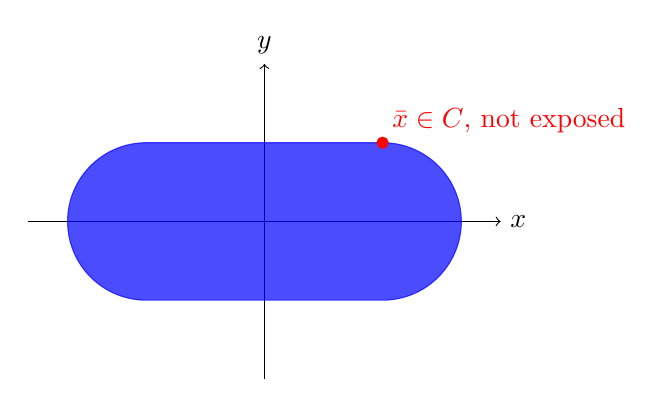
\begin{tikzpicture}
\draw[black,->] (-3,0) -- (3,0) node[right] {$x$};
\draw[black,->] (0,-2) -- (0,2) node[above] {$y$};
\draw[fill,blue,opacity=0.7] (-1.5, 1) arc (90:270:1) -- 
(1.5, -1) arc (270:450:1) -- cycle;
\draw[fill, red]
 (1.5, 1) circle (2pt) node[above right] (a) {$\bar x\in 
\ext C$, not exposed};
\end{tikzpicture}
}
\end{enumerate}
\textbf{19 ** (Tangency conditions).} Let $\Y$ be a Euclidean space. 
Fix a convex set $C$ in $\E$ and a point $x$ in $C$.
\begin{enumerate}[(a)]
\item Show $x\in \core C$ if and only if $T_C(x)=\E$. (You may 
use Exercise 20(a).) \\
\bluea{
$x\in \core C\iff \R_+(C-x)\E \iff \cl\R_+(C-x)=T_C(x)=\E$.
}
\item For a linear map $A:\E\to\Y$, prove $AT_C(x)\subset T_{AC}(Ax)$.
\bluea{
\begin{align*}
AT_C(x) &= A\cl\R_+(C-x) \subset \cl A\R_+(C-x) \\
&= \cl\R_+A(C-x) = \cl\R_+(AC-Ax) = T_{AC}(Ax).
\end{align*}
For any set $S,\; A\cl S\subset \cl AS$ because $s^i\to s
\implies As^i\to As$.
}
\item For another convex set $D$ in $\Y$ and a point $y\in D$, prove 
\begin{align*}
&N_{C\times D}(x,y) = N_C(x)\times N_D(y) \text{ and }\\
&T_{C\times D}(x,y) = T_C(x)\times T_D(y).
\end{align*}
\bluea{
Suppose $(a,b)\in N_{C\times D}(x,y)$. Then, since $x\in C$, 
for any $y'\in D,\; \ip{(a,b),(x,y')-(x,y)} = \ip{b,y'-y}\leq 0$.
Similarly because $y\in D$, $\ip{a,x-x'}\leq 0$ for any $x'\in C$. 
Thus, $(a,b)\in N_C(x)\times N_D(y)$. If $a\in N_C(x)$ and $b\in 
N_D(y)$, then  
\begin{equation*}
\forall (x',y')\in C\times D,\quad \ip{(a,b),(x',y')-(x,y)}
= \ip{a, x'-x}+\ip{b,y'-y} \leq 0.
\end{equation*}
Therefore, $N_{C\times D}(x,y) = N_C(x)\times N_D(y)$. 
\begin{align*}
T_{C\times D}(x,y) &= \cl\R_+( C\times D-(x,y)) = \cl\R_+((C-x)
\times (D-y)) \\
&=\cl(\R_+(C-x) \times \R_+(D-y)) =
 (\cl\R_+(C-x))\times (\cl\R_+(D-y)) = T_C(x)\times T_{D}(y).
\end{align*}
For the third equality, clearly $\cl\R_+(C-x)\times(D-y)
\subset \cl(\R_+(C-x)\times \R_+(D-y))$. For the other 
direction, if $\mu u\in \R_+(C-x)$ and $\nu v\in \R_+(D-y)$, 
then if $\mu=\nu=0$ clearly $(0,0)\in \R_+(C-x)\times(D-y).$
Otherwise, $\frac{\mu}{\mu+\nu}u\in C-x$ because 
$0,u\in C-x$ and $\frac{\nu}{\mu+\nu}v \in D-y$ because $0,v\in 
D-y$. Thus, $(\mu u, \nu v)\in \R_+(C-x)\times (D-y)$, multiplying
 the previous items by $\mu+\nu\in\R_+$. \\
Alternatively, by Theorem 3.3.14 (Bipolar cone), 
$T_C(x)=\cl\R_+(C-x) = (C-x)^{--} = N_C(x)^-$. By Exercise 8 (a), 
$N_{C\times D}(x,y)^- = N_C(x)^-\times N_D(y)^-$. Therefore, 
$T_{C\times D}(x,y) = T_C(x)\times T_D(y)$.
}
\item Suppose the point $x$ also lies in the convex set $G\subset\E$. 
Prove $T_C(x)-T_G(x)\subset T_{C-G}(0)$, and deduce 
\begin{equation*}
0\in\core(C-G)\iff T_C(x)-T_G(x)=\E.
\end{equation*}\\
\bluea{
For any sets $S,T,\; \cl S-\cl T\subset \cl (S-T)$. This is because 
if $s\in \cl S$ and $t\in\cl T$, there are sequences $s^i\in S$ and 
$t^i\in T$ such that $s^i-t^i\to s-t$, i.e. $s-t\in\cl(S-T)$. Thus, 
$T_C(x)-T_G(x) = \cl\R_+(C-x) - \cl\R_+(G-x) \subset \cl(\R_+(C-x)
- \R_+(G-x))$. \\
For any convex set $S$ containing 0, $x\in S\implies \lambda x
\in S$ if $\lambda\in[0,1]$. $C-x, G-s$ are convex sets containing 
0. Therefore, given $u\in C-x$, $v\in G-x$ and $\mu,\nu\in \R_+$, 
if $\mu=\nu=0$ then clearly $\mu u - \nu v = 0 \in \R_+(C-G)$.
Otherwise, 
\begin{equation*}
\mu u - \nu v = (\mu+\nu)\left(\frac{\mu}{\mu+\nu}u -\frac{\nu}{\mu
+\nu}v\right)\in\R_+(C-x - (G-x)) = \R_+(C-G).
\end{equation*}
Therefore, $T_C(x)-T_G(x)\subset \cl(\R_+(C-x)-\R_+(G-x)) = 
\cl\R_+(C-G) = T_{C-G}(0)$. \\
Alternatively, using parts (b) and (c), define the map 
$A:\E\times \E,\; (x,y)\mapsto x-y$. 
\begin{align*}
T_C(x)-T_G(x) = A(T_C(x)\times T_G(x)) = A(T_{C\times G}(x,x))
\subset T_{A(C\times G)}(x-x) = T_{C-G}(0).
\end{align*}
Now if $T_C(x)-T_G(x)=\E$, then $T_{C-G}(0) = \E$, so $0\in\core(
C-G)$. If the latter, then $T_{C-G}(0) = \E$. Inspecting (b), 
$\cl AT_C(x) = T_{AC}(Ax)$ for linear $A$ and convex $C,\,x\in C$,
so
$\cl(T_C(x)-T_G(x)) = T_{C-G}(0) = \E$, so $T_C(x)-T_G(x)=\E$ by 
(a).
}
\item Show that the condition (3.3.8) in the Fenchel theorem can be 
replaced by the condition 
\begin{equation*}
T_{\dom g}(Ax) - AT_{\dom f}(x) = \Y
\end{equation*}
for an arbitrary point $x$ in $\dom f\cap A^{-1}\dom g$.\\
\bluea{
Since by part (b), $AT_{\dom f}(x) \subset T_{A\dom f}(Ax)$, 
we have 
\begin{equation*}
\Y = T_{\dom g}(Ax)-AT_{\dom f}(x) \subset 
T_{\dom g}(Ax) - T_{A\dom f}(Ax) \implies T_{\dom g}(Ax)
- T_{A\dom f}(Ax) = \Y.
\end{equation*}
By part (d), this implies $0\in\core(\dom g - A\dom f)$.
}
\end{enumerate}
\textbf{20 ** (Properties of the relative interior).} (We 
use Exercise 9 (Open mapping theorem), as well as Section 1.1, 
Exercise 13.)
\begin{enumerate}[(a)]
\item Let $D$ be a nonempty convex set in $\E$. Prove $D$ is a 
linear subspace if and only if $\cl D$ is a linear subspace. 
(Hint: $\ri D\neq\emptyset.$)\\
\bluea{
If $D$ is a linear subspace, then since linear subspaces are closed, 
$\cl D$ is a linear subspace. \\
Now suppose $\cl D$ is a linear subspace, and suppose $v\in \cl D$.
If $v\notin \aff D$, then since $\aff D$ is closed and convex, 
$v$ has a positive distance to $\aff D$. But, $D\subset \aff D$, 
and there is a sequence in $D$ converging to $v$, contradiction. 
Thus, $v\in \aff D$. In particular, $0\in \aff D$, so 
$\aff D = \spn D$.\\
By section 1.1 Exercise 13 (b), $\ri D$ is nonempty. Let $x\in\ri D$.
There exists $\ve>0$ such that 
for any $v\in \aff(D)-x = \aff(D)-0 = \spn(D)$ where $\|v\|\leq \ve,
\; x+v\in D$. 
Now let $y\in \cl D$ be arbitrary. Since $x\in\cl D$ and $\cl D$ 
is linear, $x+y\in\cl D$. Then, there is an element $u\in D$ 
$\ve$ close to $x+y$. Define $\eta = u-(x+y)$. Since $\|\eta\|\leq 
\ve$, we have $x-\eta\in D$. By convexity of $D$, 
\begin{equation*}
\frac{1}{2}u + \frac{1}{2}(x-\eta) 
= \frac{1}{2}(x+y+\eta) + \frac{1}{2}(x-\eta)
= x+\frac{1}{2}y \in D.
\end{equation*}
Since $y\in \cl D$, a linear space containing $x$, was arbitrary, 
$y=2(z-x)$ for arbitrary $z\in\cl D$ shows that $\cl D\subset D$. 
I.e., $D$ is a linear subspace.
This finishes the proof.
}
\item For a point $x$ in a convex set $C\subset\E$, prove the 
following properties are equivalent:
\begin{enumerate}[(i)]
\item $x\in \ri C$. \\
\bluea{
(i)$\implies$(ii): By Section 1.1 Exercise 13 (d), $x\in\ri C$
implies $\R_+(C-x)$ is a linear subspace. Since linear subspaces
are closed $\cl\R_+(C-x) = \R_+(C-x)$ is a linear subspace.
}
\item The tangent cone $\cl\R_+(C-x)$ is a linear subspace.\\
\bluea{
(ii)$\implies$(iii): Since $N_C(x) = (\cl\R_+(C-x))^-
= (T_C(x))^-$,  
$N_C(x)=\{\phi : \ip{\phi, z}\leq 0 \text{ for all }z\in T_C(x)\}$. 
If $\ip{\phi, z} < 0$, then $\ip{\phi, -z}>0$ and $-z\in T_C(x)$ 
since $T_C(x)$ is a linear subspace, i.e. $\phi\notin N_C(x)$. 
Thus, $N_C(x) = \{\phi: \ip{\phi, z} = 0 \text{ for all }z\in T_C(x)\}
= T_C(x)^{\perp}$, the orthogonal complement of $T_C(x)$, which is a
linear subspace.
}\vspace{-0.15in}
\item The normal cone $N_C(x)$ is a linear subspace.  \\
\bluea{
(iii)$\implies$(iv): Being a convex cone closed under negation 
implies being a linear subspace, since convex cones are closed 
under addition of nonnegative multiples.
}
\item $y\in N_C(x)\Ra -y\in N_C(x)$. \\
\bluea{
(iv)$\implies$(i): (iv) implies that $N_C(x) = \{\phi\in\E:
\ip{\phi, z} =0 \; \forall z\in C-x\}$. Since the condition 
$\ip{\cdot, z}=0$ is closed under linear combinations, $N_C(x)$ 
is linear. Thus, $\cl(\R_+(C-x)) = N_C(x)^-=N_C(x)^\perp$ is linear. 
Thus, by part (a)
$\R_+(C-x)$ is linear. Thus, by Section 1.1 Exercise 13 (d),
$x\in\ri C$.
}
\end{enumerate}
\item For a convex set $C\subset\E$ and a linear map $A:\E\to\Y$, 
prove $A\ri C\supset \ri AC$, and deduce 
\begin{equation*}
A\ri C = \ri AC.
\end{equation*}
\green{I found this question difficult\ldots}\\
\bluea{
Suppose $y\in\ri AC$. Denote $C\cap A^{-1}y = \{x\in C: Ax=y\}$
and take $\bar x\in \ri(C\cap A^{-1}y)$. We will show that 
$\bar x\in\ri C$, which would imply $y\in A\ri C$ since $A\bar x
= y$ by definition of $C\cap A^{-1}y$. We will do so by 
showing condition (iv) from the previous part. \\
Using the fundamental theorem of linear algebra, we can express
an arbitrary element of $N_C(\bar x)$ as $A^*\phi + w$, where 
$w\in \nul(A)$. For any $x'\in C$, we have 
\begin{equation}
\label{ncon}
\ip{\phi, Ax'-y} + \ip{w, x'-\bar x} 
=\ip{A^*\phi + w, x'-\bar x}  \leq 0.
\end{equation}
For any $x'\in C\cap A^{-1}y$, this says $\ip{w,x'-\bar x}\leq 0$, 
i.e. $w\in N_{C\cap A^{-1}y}(\bar x)$. Since $\bar x\in\ri(C\cap 
A^{-1})$, $-w\in N_{C\cap A^{-1}y}(\bar x)$, i.e. $\ip{w,x'-\bar x}
= 0$ for every $x'\in C\cap A^{-1}y$. \\
Now since $y\in \ri AC$, for any $z\in AC$, there exists $\epsilon > 0$
such that $y+\epsilon(y-z)\in AC$ (See Section 1.1 Exercise 13 (d)).
So there exist $x',\tilde x\in C$ where $Ax'=z$ and $A\tilde x = 
y+\epsilon(y-z)$. Now observe that 
\begin{equation*}
A\left(\frac{\epsilon}{1+\epsilon}x' + \frac{1}{1+\epsilon}\tilde x
\right) = \frac{\epsilon}{1+\epsilon}z + \frac{1}{1+\epsilon}(y
+ \epsilon(y-z)) = y \implies \frac{\epsilon}{1+\epsilon}x' 
+ \frac{1}{1+\epsilon}\tilde x \in C\cap A^{-1}y.
\end{equation*}
Furthermore, applying \eqref{ncon} to $x'$ and $\tilde x$, we get 
\begin{equation*}
Q_1:= \ip{\phi, z-y} + \ip{w, x'-\bar x} \leq0 ,\qquad 
Q_2:=\epsilon\ip{\phi, y-z} + \ip{w, \tilde x - \bar x} \leq 0.
\end{equation*}
But in fact, if we add the left hand sides, scaled by $\epsilon/(1+
\epsilon)$ and $1/(1+\epsilon)$, 
\begin{equation*}
\frac{\epsilon}{1+\epsilon}Q_1 + \frac{1}{1+\epsilon}Q_2 = 
\ip{w, \frac{\epsilon}{1+\epsilon}x' + \frac{1}{1+\epsilon}\tilde x}
= 0
\end{equation*}
because $\epsilon x'/(1+\epsilon) + \tilde x/(1+\epsilon)\in C\cap
A^{-1}y$. We added together two nonpositive things and produced 
zero; therefore, they must both equal 0. Since $x'$ was essentially
arbitrary (we took arbitrary $z\in AC$, and arbitrary $x'\in C$
where $Ax'=z$), we have $\ip{A^*\phi+w, x'-\bar x} = 0$ 
for all $x'\in C$. Thus, $-(A^*\phi+w)\in N_C(\bar x)$. Thus, 
by part (b), $\bar x\in \ri C$. Since part (e) of Section 1.1,
Exercise 13 shows $A\ri C\subset \ri AC,\; A\ri C=\ri AC$.
}
\item Suppose $U$ and $V$ are convex sets in $\E$. Deduce 
\begin{equation*}
\ri(U-V)=\ri U-\ri V. 
\end{equation*}
\bluea{
Use part (c) with the linear map $A:\E\times \E,\, (x,y)\mapsto 
x-y$ and convex set $U\times V$.}
\item Apply Section 3.1, Exercise 29 (Relativizing the Max formula)
to conclude that the condition (3.3.8) in the Fenchel theorem 
(3.3.5) can be replaced by 
\begin{equation*}
\ri(\dom g)\cap A\ri(\dom f)\neq\emptyset.
\end{equation*}
\bluea{
The proof of the Fenchel theorem hinges on the existence of 
a subgradient of $h(u) = \inf_{x\in\E}\{f(x)+ g(Ax+u)\}$ at 0, which 
holds if $0\in\core(\dom h) = \core(\dom g - A\dom f)$. Section 
3.1, Exercise 29 shows that a subgradient exists if $0\in 
\ri(\dom h) = \ri(\dom g - A\dom f)$. By part (d) and (c),
this equals $0\in \ri(\dom g) - \ri(A\dom f) = \ri(\dom g) - 
A\ri(\dom f)$. I.e., $\ri(\dom g)\cap A\ri(\dom f)\neq \emptyset$.
}
\item Suppose the function $f:\E\to(-\infty,+\infty]$ is bounded below
on the convex set $C\subset\E$, and $\ri C\cap\ri(\dom f)\neq 
\emptyset$. Prove there is an affine function $\alpha\leq f$ with 
$\inf_C f = \inf_C\alpha$.\\
\bluea{
By $\ri C\cap \ri(\dom f)\neq \emptyset$ and $f$ being bounded 
below on $C$, the following problems equal and have finite value:
\begin{align*}
\inf_{x\in C}\{f(x)\} &= \sup_{\phi\in\E}\{-f^*(\phi) - \delta_C^*(
-\phi)\} \\
&= \sup_{\phi\in \E}\{-\sup_{x'\in\E}\{\ip{\phi, x'}-f(x')\}
- \sup_{x\in C}\ip{-\phi, x}\} \\
&= \sup_{\phi\in\E}\{\inf_{x'\in\E}\{f(x')-\ip{\phi, x'}\}
+ \inf_{x\in C}\ip{\phi, x}\}.
\end{align*}
Moreover, the $\sup$ is obtained by some $\phi\in\E$, so that 
\begin{equation*}
\inf_{x\in C} f(x)  = \inf_{x'\in\E}\{f(x') - \ip{\phi, x'}\}
+ \inf_{x\in C}\ip{\phi, x}.
\end{equation*}
In other words, $\inf_C f = \inf_C \alpha$ for the affine 
$\alpha = \inf_{x'\in\E}\{f(x')-\ip{\phi, x'}\} + \ip{\phi, \cdot}$. 
Moreover, by definition 
\begin{equation*}
\alpha(x) = \ip{\phi, x} + \inf_{x'\in\E}\{f(x')-\ip{\phi, x'}\}
\leq \ip{\phi, x}+f(x)-\ip{\phi, x} = f(x).
\end{equation*}
}
\end{enumerate}
\noindent
\textbf{21 ** (Essential smoothness).} For any convex $f$ and any 
point $x\in\bd(\dom f)$, prove $\partial f(x)$ is either empty or 
unbounded. Deduce that a function is essentially smooth if and only 
if its subdifferential is always singleton or empty.
\bluea{
\begin{proof}
If $\phi\in\partial f(x)$, then for any $d\in N_{\dom f}(x)$ and 
$x'\in \dom f$, 
\begin{equation*}
\ip{\phi + d, x'-x} \leq \ip{\phi, x'-x}\leq f(x')-f(x),
\end{equation*}
proving that $\phi+d\in \partial f(x)$. If $x\in\bd(\dom f)$, then 
$x\notin \inter(\dom f) = \core(\dom f)$ by Theorem 4.1.4 (Core 
and interior). Thus, $\R_+(\dom f - x)\neq \E$. Thus, 
$T_{\dom f}(x) \neq \E$. Thus, $N_{\dom f}(x) \neq \{0\}$. 
Thus, $N_{\dom f}$ is unbounded, which implies $\partial f(x)$ is 
unbounded if nonempty.\\
Since $\dom\partial f\subset \core(\dom f)$ for essentially 
smooth $f$, (see proof of 
Section 3.1 Exercise 24), we can apply the max formula (Theorem 
3.1.8) to any point $\bar x\in\dom\partial f$ to show that 
$\partial f(\bar x)$ is a singleton.
 \green{Did I overkill the convex analysis? XD}
\end{proof}}
\noindent
\textbf{22 ** (Birkhoff's theorem [15])} We use the notation of 
Section 1.2.
\begin{enumerate}[(a)]
\item Prove $\P^n = \{(z_{ij})\in\Gamma^n \mid z_{ij}=0\text{ or }
1 \text{ for all }i,j\}.$  \\
\bluea{
The provided definition of $\P^n$ is that each entry is 0 or 1 
and each row and each column contains one 1. If $X\in\P^n$, 
clearly it is doubly stochastic and 0-1, showing $\subset$. 
If on the other hand, $X$ is 0-1 and doubly stochastic, each 
row and column contains exactly one 1, since if some row/column 
contains 0 ones, the sum is $0<1$, and if it contains more than 
one 1, the sum is strictly greater than 1. This proves $\supset$.
}
\item Prove $\P^n \subset\ext(\Gamma^n)$. \\
\bluea{
If $\lambda\in(0,1)$ and $X_1 \neq X_2\in \Gamma^n,\; X\in\P^n$,
$\lambda X_1 + (1-\lambda)X_2\neq X$ because $\lambda X_1 + 
(1-\lambda)X_2 \notin \P^n$: if $\lambda X_1 + (1-\lambda)X_2$ 
is 0-1, then $X_1$ and $X_2$ are both 0-1 (or else some entry 
is in $(0,1)$), and have ones in the same places for the same 
reason. In other words, $X_1=X_2$, a contradiction. Thus, 
$X\in\ext(\Gamma^n)$.
}
\item Suppose $(z_{ij})\in \Gamma^n\setminus \P^n$. Prove there 
exist sequences of distinct indices $i_1, i_2,\ldots, i_m$ and 
$j_1,j_2,\ldots, j_m$ such that 
\begin{equation*}
0< z_{i_r,j_r}, z_{i_{r+1}, j_r} < 1 \quad (r=1,2,\ldots, m)
\end{equation*}
(where $i_{m+1}=i_1)$). For these sequences, show the matrix 
$(z_{i,j}')$ defined by 
\begin{equation*}
z_{ij}' - z_{ij} = \begin{cases} \epsilon & \text{if } (i,j)=
(i_r,j_r)\text{ for some } r\\
-\epsilon & \text{if }(i,j) = (i_{r+1}, j_r)\text{ for some } r\\
0 & \text{otherwise}
\end{cases}
\end{equation*}
is doubly stochastic for all small real $\epsilon$. Deduce 
$(z_{ij})\notin\ext(\Gamma^n)$. \\
\bluea{
Since $(z_{ij})\notin \P^n$, we can find $(i_1, j_1)$ such that 
$z_{i_1, j_1}\in (0,1)$. Since $(z_{ij})\in \Gamma^n$, there 
must be $(i_2, j_1)$ with $z_{i_2, j_1}\in (0,1)$ (the $j_1$ 
column sums to 1). Since the $i_2$ row sums to 1, there 
must be $(i_2, j_2)$ with $z_{i_2, j_2}\in (0,1)$. Since 
the $j_2$ column sums to 1, we can find $(i_3, j_2),\ldots$. 
This gives a sequence 
\begin{align*}
S=(i_1,j_1), (i_2,j_1), (i_2,j_2), (i_3, j_2), (i_3, j_3), \ldots
\qquad (i,j)\in S\implies z_{ij}\in(0,1).
\end{align*}
Suppose that $(i_n)$ repeats at or before $(j_n)$ repeats. That 
is, there exist $k<l$ with $i_k=i_l$ and $j_n \neq j_m$ for all 
$n,m < l$. Consider the subsequence 
\begin{equation*}
(i_k, j_k), (i_{k+1},j_k),
\ldots, (i_{l-1}, j_{l-1}), (i_k=i_l, j_{l-1}).
\end{equation*}
 By construction, $i_{k+1}\neq i_{k}$, so $l>k+1$ and $i_k,
\ldots, i_{l-1}$ and $j_k,\ldots, j_{l-1}$ are sequences of 
distinct elements of length at least 2. The exhibited subsequence
demonstrates that these sequences fit the desired requirements. \\
Now suppose that $(j_n)$ repeats before $(i_n)$ does. Then for 
some $k<l,\, j_k=j_l$ and $i_1,\ldots, i_l$ are distinct. 
Similarly by construction $j_k \neq j_{k+1}$ so $l>k+1$. Consider 
\begin{equation*}
(i_{k+1}, j_k=j_l), (i_{k+1}, j_{k+1}), \ldots, (i_l, j_l=j_k).
\end{equation*}
This subsequence shows that $i_{k+1}, \ldots, i_l$ and 
$j_{k+1},\ldots, j_l$ are sequences of distinct elements of 
length at least 2 satisfying the desired properties. \\
Now since each row and column of $z_{ij}'-z_{ij}$ sums to 0 
(they are either 0 or have an $\epsilon$ and a $-\epsilon$), 
for $|\epsilon|$ small enough $z_{ij}'$ is doubly stochastic. 
Thus, $(z_{ij})\notin\ext(\Gamma^n)$.
}
\item Deduce $\ext(\Gamma^n)=\P^n$. Deduce Birkhoff's theorem 
(1.2.5). \\
\bluea{
By part (b), $\P^n\subset \ext(\Gamma^n)$ and by part (c), 
$\ext(\Gamma^n)\subset\P^n$. Thus $\ext(\Gamma^n) = \P^n$. 
By Theorem 4.1.8 (Minkowski) and compact convexity of $\Gamma^n$,
$\Gamma^n = \conv(\P^n)$, which is Birkhoff's theorem.
}
\item Use Caratheodory's theorem (Section 2.2, Exercise 5) to 
bound the number of permutation matrices needed to represent a 
doubly stochastic matrix in Birkhoff's theorem. \\
\bluea{
Caratheodory's theorem states that any element in the convex 
hull of $\ip{a^i\mid i\in I}$ can be expressed as a convex 
combination of elements in some $J\subset I$ where $|J|\leq 
1 + \dim\E$. The dimension of $\R^{n\times n}\supset 
\P^n$ is $n^2$ and $\conv(\P^n) = \Gamma^n$, so any doubly 
stochastic matrix can be represented by $n^2+1$ permutation
matrices. (Actually $\dim\spn(\P^2) = 2$, and any linear 
combination of permutation matrices have row and column sums 
identical, i.e. $X\vec 1 = X^\top\vec 1 = c\vec 1$ for some 
$c\in\R$, so it's smaller XD).
}
\end{enumerate}
\end{document}
